\chapter{Tecnologías de conversión}
\label{cap:conversion}

La biomasa puede transformarse en calor, electricidad y combustibles secundarios mediante diversos procesos tecnológicos. La selección de la ruta adecuada depende principalmente de la humedad de la materia prima, su composición lignocelulósica, el contenido de cenizas, la escala de potencia y el vector energético requerido \cite{balopi2025review, irena2015heatpower}.

\section{Rutas de conversión de la biomasa}
\label{sec:rutas}

El aprovechamiento tradicional (fogones abiertos de leña y carboneras rudimentarias) presenta eficiencias muy bajas, del orden de 10--20~\%, y genera severa contaminación intradomiciliaria. Por el contrario, la bioenergía moderna emplea equipos controlados de alta eficiencia y tratamiento de emisiones. Las tecnologías modernas se agrupan en tres grandes familias: procesos \textbf{termoquímicos}, \textbf{bioquímicos} y \textbf{fisicoquímicos} (Tabla~\ref{tab:rutas_conversion}). En los procesos termoquímicos, la relación de equivalencia de aire ($\lambda$, razón entre el aire suministrado y el estequiométrico) define el régimen operativo: combustión ($\lambda > 1$), gasificación ($\lambda \approx 0{,}2\text{--}0{,}4$) y pirólisis ($\lambda = 0$).

\begin{table}[htbp]
\centering
\small
\caption{Rutas modernas de conversión de la biomasa ($\lambda$: relación aire suministrado / aire estequiométrico).}
\label{tab:rutas_conversion}
\begin{tabularx}{\textwidth}{@{}p{2.0cm} p{2.7cm} X p{2.8cm} p{2.6cm}@{}}
\toprule
\textbf{Ruta} & \textbf{Proceso} & \textbf{Condición clave} & \textbf{Producto principal} & \textbf{Uso en potencia} \\
\midrule
Termoquímica & Combustión & Exceso de aire ($\lambda > 1$); 800--1\,000~\textdegree C o más & Gases calientes $\rightarrow$ vapor & Ciclo Rankine, ORC \\
Termoquímica & Gasificación & Aire subestequiométrico ($\lambda \approx 0{,}2\text{--}0{,}4$); 700--1\,000~\textdegree C & Syngas ($\mathrm{CO}$, $\mathrm{H_2}$, $\mathrm{CH_4}$) & Motor o turbina de gas \\
Termoquímica & Pirólisis & Sin oxígeno ($\lambda = 0$); 300--600~\textdegree C & Bio-oil, biochar, gas & Calderas, motores adaptados \\
Bioquímica & Digestión anaeróbica & Sin oxígeno; 35--55~\textdegree C; microorganismos & Biogás (50--70~\% $\mathrm{CH_4}$) & Motogenerador \\
Bioquímica & Fermentación alcohólica & Levaduras sobre azúcares & Bioetanol & Transporte (principalmente) \\
Fisicoquímica & Extracción + transesterificación & Aceite + alcohol + catalizador & Biodiésel & Transporte (principalmente) \\
\bottomrule
\end{tabularx}
\end{table}

\begin{figure}[H]
    \centering
    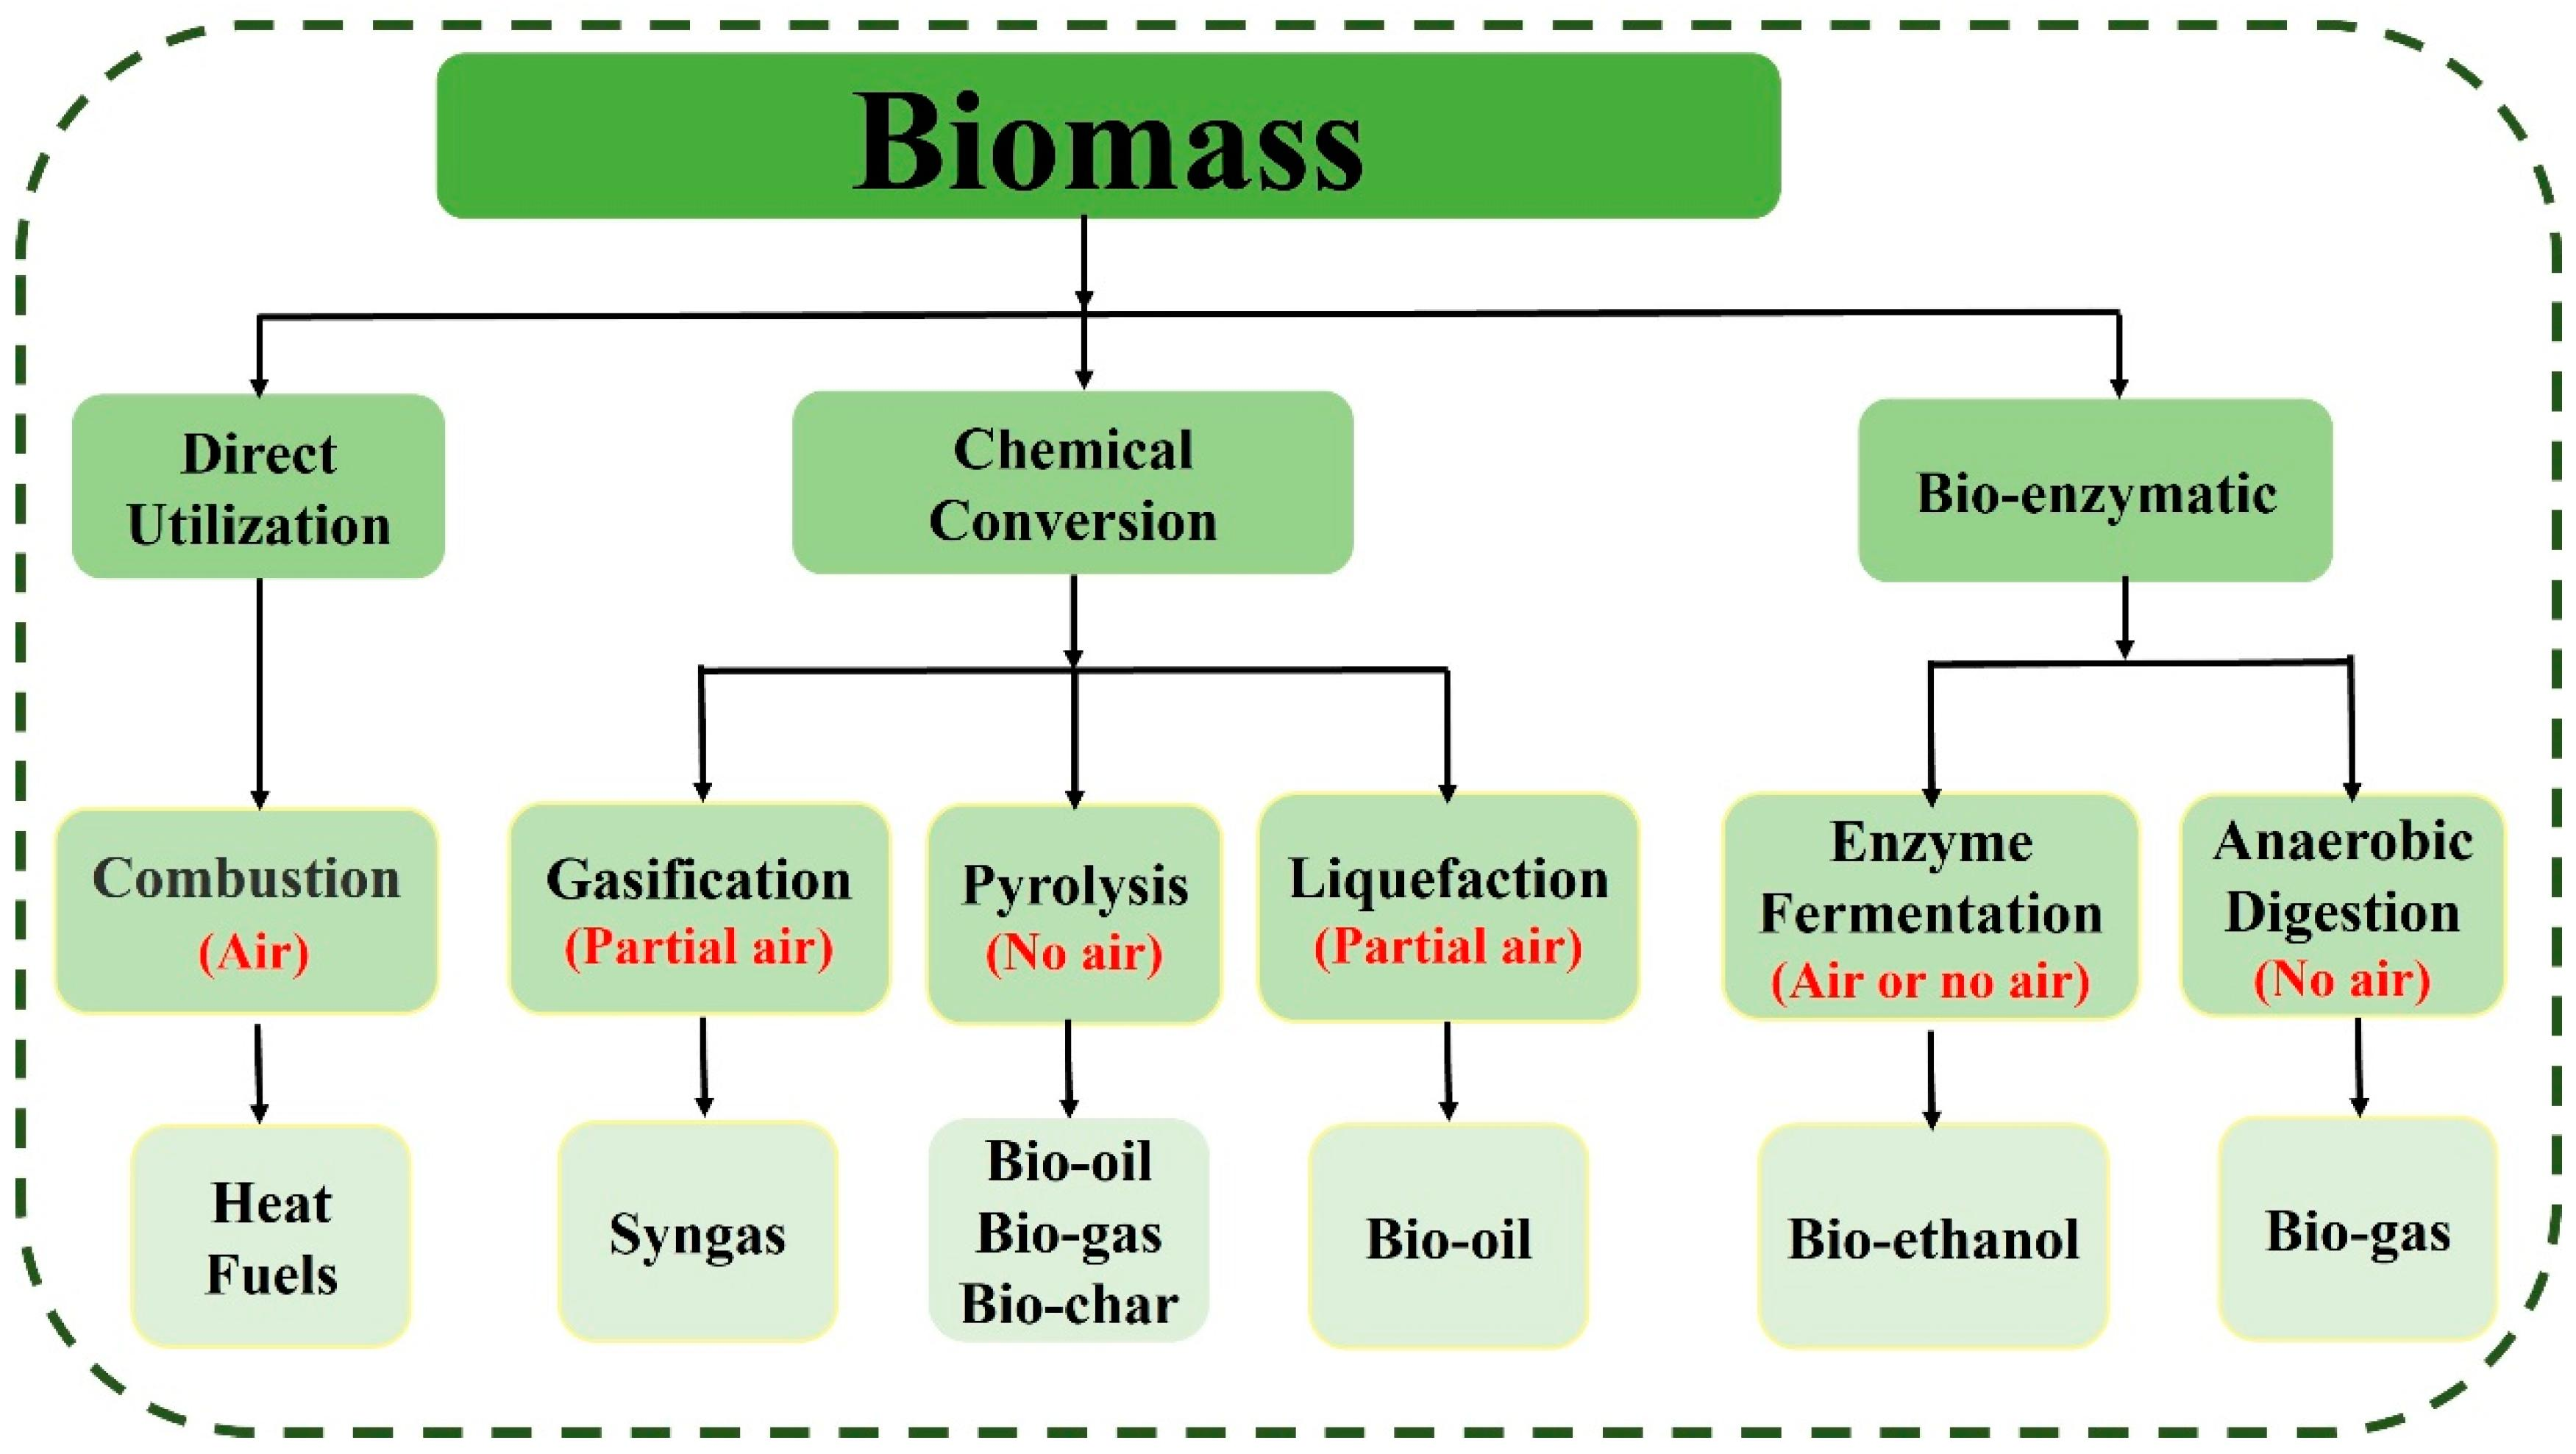
\includegraphics[width=0.9\textwidth]{Figuras/Sección B - Tecnologías de Conversión/Tecnologías de Conversión.jpg}
    \caption{Principales rutas de transformación de la biomasa en productos energéticos. Cada ruta depende de la naturaleza de la materia prima y del producto que se desea obtener}
\end{figure}

\section{Combustión directa}
\label{sec:combustion}

La combustión directa es la ruta tecnológica dominante y representa más del 90~\% de la contribución global de la bioenergía \cite{vanloo2007handbook}. Consiste en la oxidación completa de la biomasa con exceso de aire para liberar energía térmica, la cual se transfiere en una caldera para generar vapor destinado a procesos industriales o a la expansión en una turbina.

\subsection{Mecanismo y control de emisiones}
Dentro del hogar de la caldera, cada partícula de biomasa atraviesa cuatro etapas que ocurren de forma simultánea en distintas zonas:
\begin{enumerate}[leftmargin=1.5em]
\item \textbf{Calentamiento y secado} (hasta $\sim$100--150~\textdegree C): evaporación endotérmica de la humedad.
\item \textbf{Devolatilización} ($\sim$200--500~\textdegree C): liberación de materia volátil ($\mathrm{CO}$, $\mathrm{H_2}$, $\mathrm{CH_4}$, hidrocarburos y alquitranes), equivalente al 70--85~\% de la masa seca.
\item \textbf{Combustión de los volátiles} en fase gaseosa: forma la llama y libera la mayor fracción del calor.
\item \textbf{Combustión del carbonizado} (\textit{char}) en la superficie de la partícula, etapa más lenta que deja como residuo la ceniza.
\end{enumerate}

De forma global, la reacción de oxidación completa con aire puede representarse como:
\begin{equation}
\mathrm{CH}_x\mathrm{O}_y + a\left(\mathrm{O_2} + 3{,}76\,\mathrm{N_2}\right) \longrightarrow \mathrm{CO_2} + \mathrm{H_2O} + \mathrm{N_2} + \text{calor}
\end{equation}
Una combustión eficiente exige cumplir las denominadas «tres T»: \textit{temperatura} suficiente, \textit{tiempo de residencia} adecuado y \textit{turbulencia} para mezclar aire y gases. El aire se suministra escalonado en aire primario (bajo la parrilla o el lecho) y aire secundario (sobre el lecho, para quemar los volátiles), con excesos de aire típicos de 20--60~\%. Los principales contaminantes y sus sistemas de control se resumen en la Tabla~\ref{tab:emisiones_combustion}.

\begin{figure}[H]
    \centering
    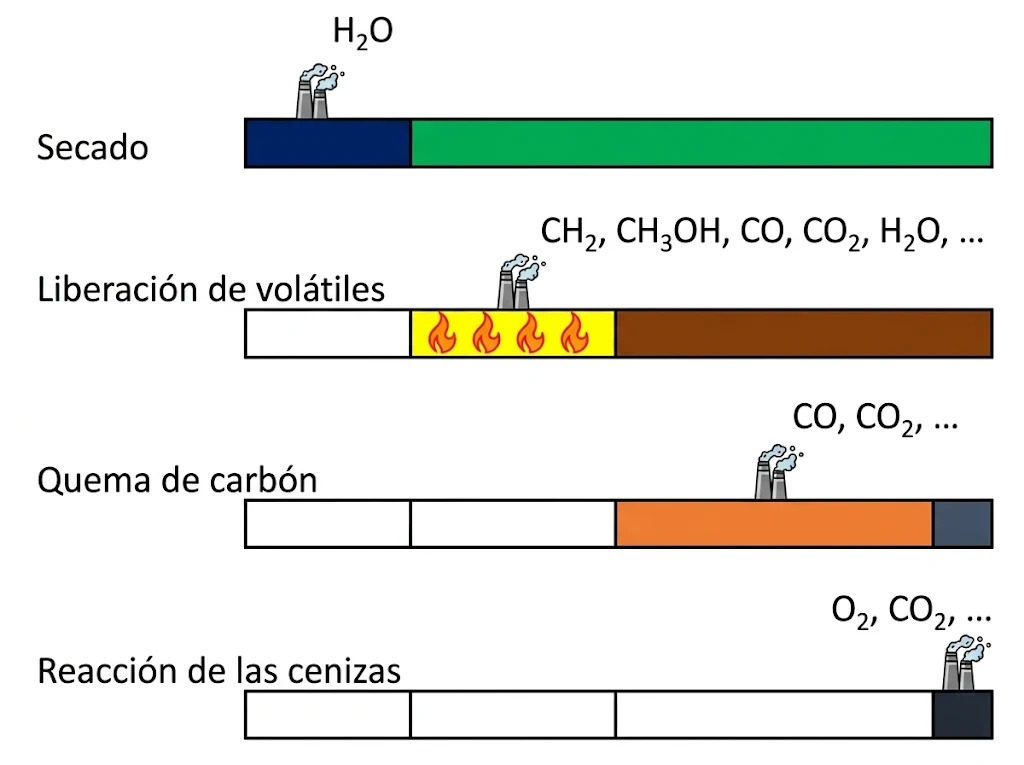
\includegraphics[width=0.9\textwidth]{Figuras/Sección B - Tecnologías de Conversión/Etapas de combustión de una partícula de biomasa.jpg}
    \caption{Etapas de secado, liberación de volátiles, combustión del carbonizado y formación de cenizas. Es la imagen más directamente relacionada con la explicación de tu mecanismo de combustión}
\end{figure}

\begin{table}[htbp]
\centering
\caption{Principales emisiones de la combustión de biomasa y tecnologías de control.}
\label{tab:emisiones_combustion}
\begin{tabularx}{\textwidth}{@{}l X X@{}}
\toprule
\textbf{Contaminante} & \textbf{Origen} & \textbf{Medidas de control} \\
\midrule
Material particulado & Cenizas volantes y aerosoles de sales alcalinas & Ciclones (partículas gruesas), filtros de mangas o precipitadores electrostáticos (partículas finas). \\
$\mathrm{CO}$ e hidrocarburos & Combustión incompleta por falta de aire, mala mezcla o baja temperatura & Aire secundario bien distribuido, control de exceso de aire (sonda $\mathrm{O_2}$) y tiempo de residencia. \\
$\mathrm{NO}_x$ & Principalmente nitrógeno del propio combustible ($\mathrm{NO}_x$ combustible) & Combustión por etapas, recirculación de gases, reducción selectiva no catalítica (SNCR con amoníaco o urea) o SCR. \\
$\mathrm{SO_2}$ y $\mathrm{HCl}$ & Azufre y cloro del combustible (bajos en madera, mayores en pajas) & Adición de caliza en el lecho o inyección de sorbentes secos. \\
\bottomrule
\end{tabularx}
\end{table}

\subsection{Equipos de combustión}
Las calderas industriales de biomasa se clasifican según la tecnología de hogar empleada (Tabla~\ref{tab:tecnologias_combustion}). Los lechos fluidizados circulantes (CFB) permiten unidades individuales mucho mayores que los burbujeantes (BFB), del orden de $300~\mathrm{MW_e}$ frente a $\sim 100~\mathrm{MW_e}$, con mayor flexibilidad de combustible \cite{flynn2005alholmens, irena2015heatpower}.

\begin{table}[htbp]
\centering
\caption{Tecnologías de combustión directa de biomasa \cite{irena2015heatpower, vanloo2007handbook}.}
\label{tab:tecnologias_combustion}
\begin{tabularx}{\textwidth}{@{}l l X X@{}}
\toprule
\textbf{Tecnología} & \textbf{Escala típica} & \textbf{Ventajas} & \textbf{Limitaciones} \\
\midrule
Parrilla fija & Pequeña & Simple y de bajo costo de inversión. & Exige combustible homogéneo; control limitado. \\
Parrilla móvil, vibratoria o inclinada & Pequeña a mediana & Madura para residuos de madera y bagazo; tolera combustibles húmedos. & Eficiencia y flexibilidad térmica intermedias. \\
Lecho fluidizado burbujeante (BFB) & Mediana & Excelente transferencia térmica; baja temperatura (800--900~\textdegree C) y menor $\mathrm{NO}_x$; admite combustibles heterogéneos. & Riesgo de aglomeración del lecho de arena con cenizas alcalinas. \\
Lecho fluidizado circulante (CFB) & Grande & Máxima flexibilidad de combustible y alta eficiencia en unidades de cientos de $\mathrm{MW_e}$. & Mayor costo de capital, consumo auxiliar y erosión interna. \\
Combustión pulverizada & Muy grande & Aprovecha calderas de carbón existentes; base de la co-combustión. & Requiere biomasa finamente molida o pellets. \\
\bottomrule
\end{tabularx}
\end{table}

\subsection{La caldera, balance global y ciclos de potencia}
La caldera integra el hogar, paredes de agua, sobrecalentador, economizador y precalentador de aire. Su eficiencia térmica sobre el PCI se sitúa entre 80 y 90~\%:
\begin{equation}
\eta_{\mathrm{caldera}} = \frac{\dot{Q}_{\text{útil}}}{\dot{m}_{\mathrm{comb}} \cdot \mathrm{PCI}}
\end{equation}

\begin{figure}[H]
    \centering
    \begin{subfigure}[b]{0.48\textwidth}
        \centering
        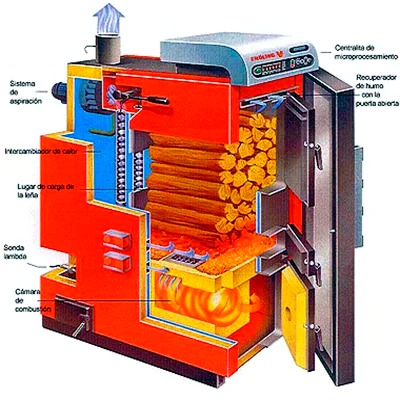
\includegraphics[width=\textwidth]{Figuras/Sección B - Tecnologías de Conversión/Combustión directa - CALDERA.jpg}
        \caption{Esquema de una caldera de combustión invertida para leña con sistema de tiro inducido, regulación por sonda lambda e intercambiador de calor vertical}
    \end{subfigure}
    \hfill
    \begin{subfigure}[b]{0.48\textwidth}
        \centering
        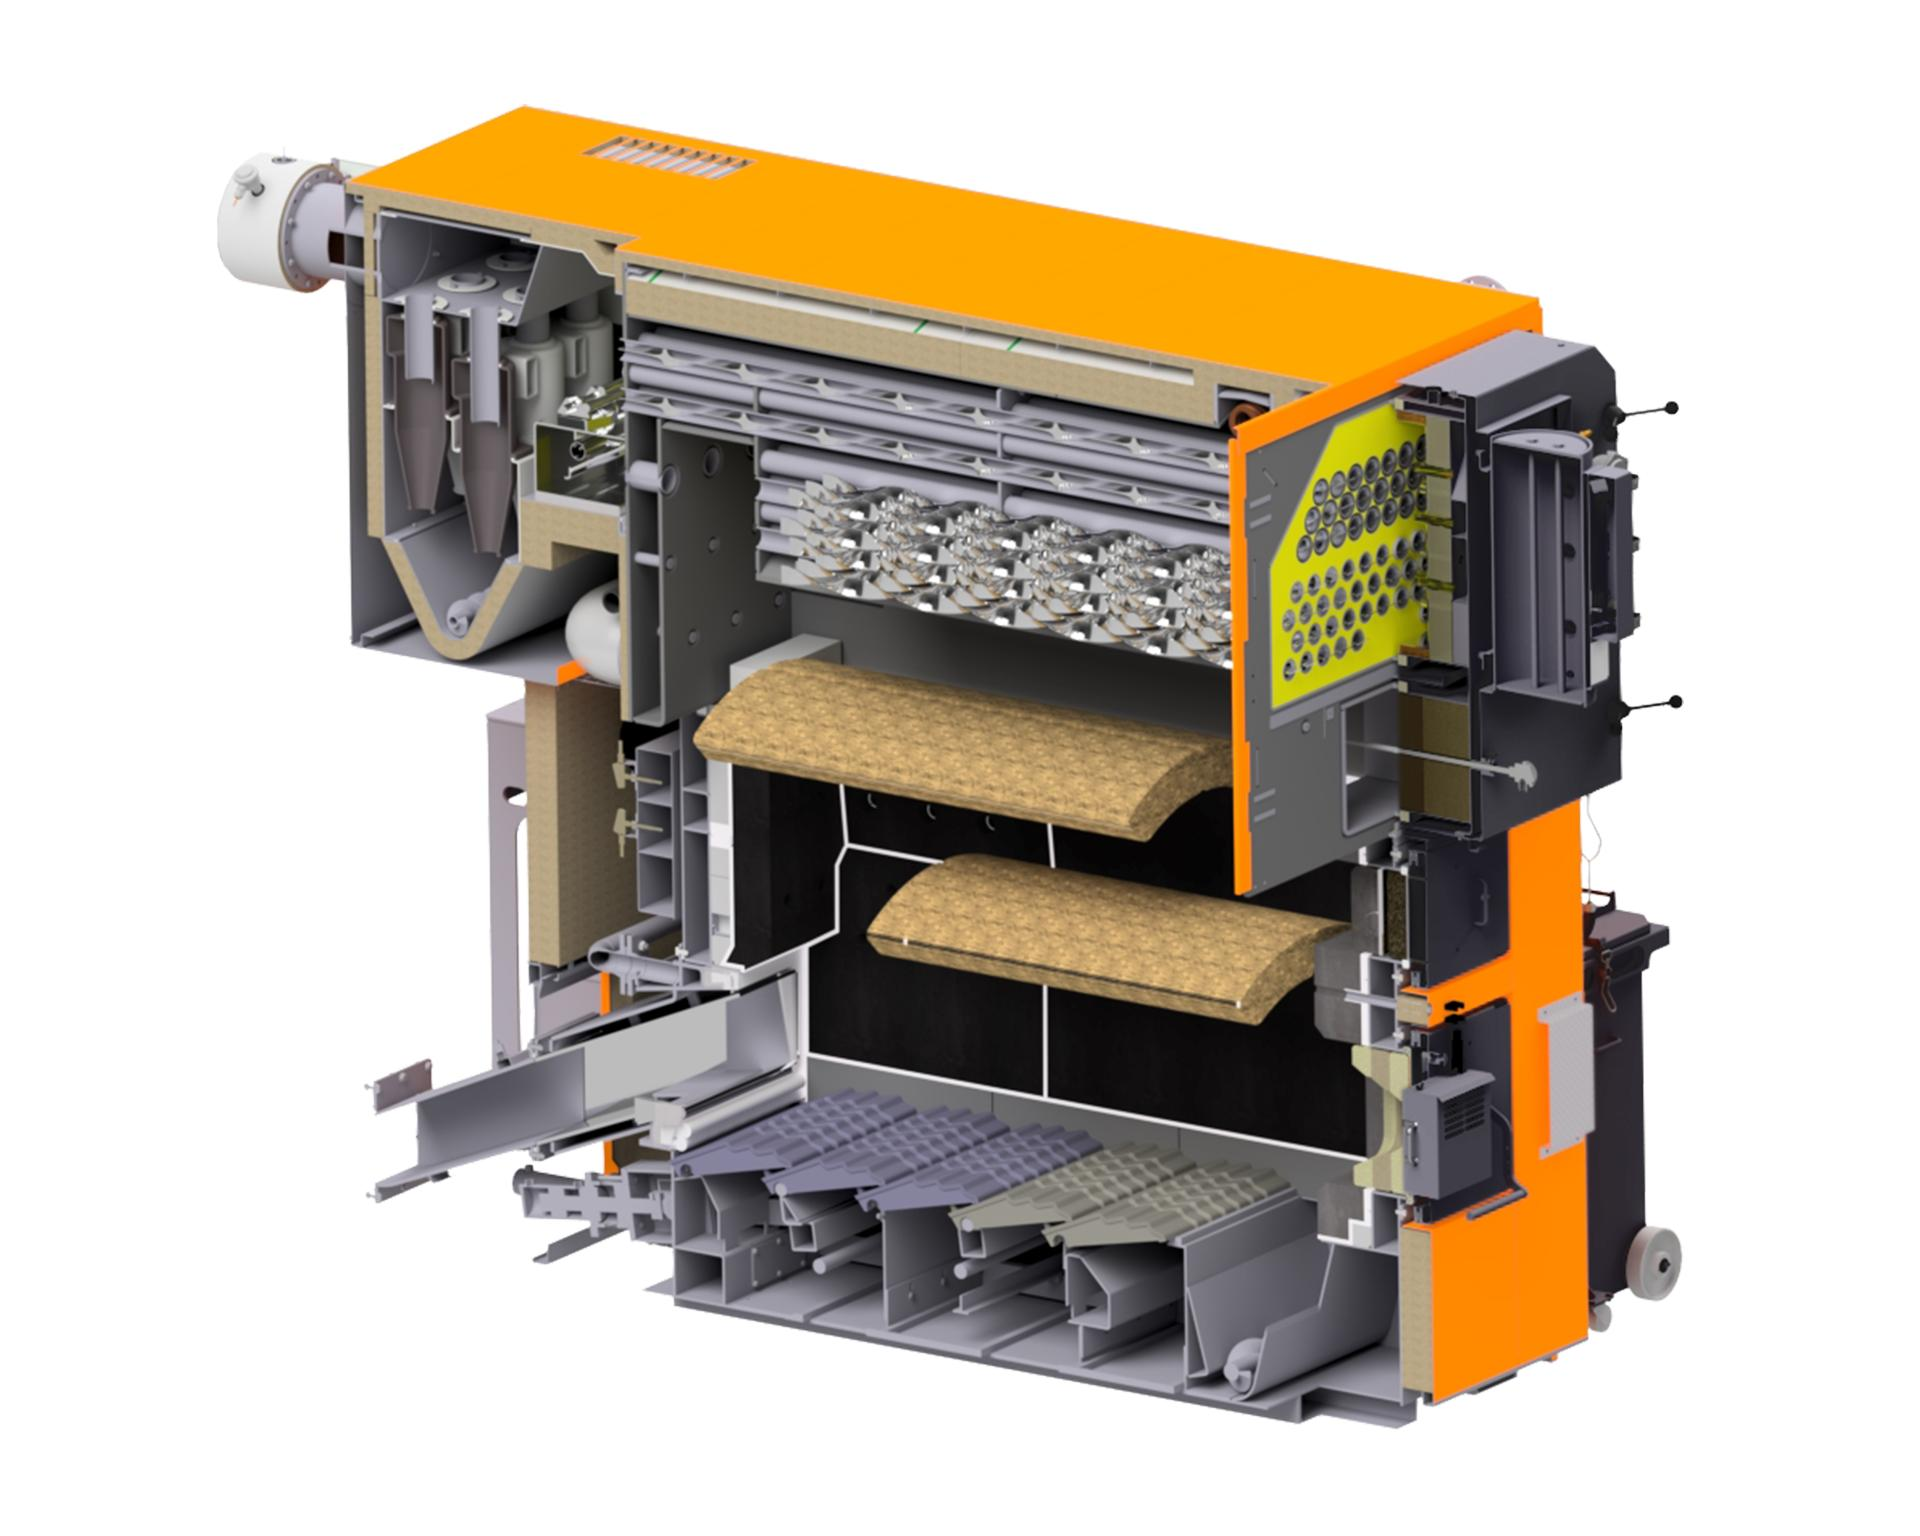
\includegraphics[width=\textwidth]{Figuras/Sección B - Tecnologías de Conversión/Combustión directa - Combustión en parrilla.jpg}
        \caption{Caldera de biomasa de parrilla escalonada móvil con bóvedas refractarias, intercambiador pirotubular horizontal y separador multiciclónico integrado}
    \end{subfigure}

    \caption{Tecnologías de calderas empleadas en la combustión directa de biomasa sólida}
    \label{fig:grupo_tres}
\end{figure}

Las principales pérdidas corresponden a los gases secos de chimenea (la mayor pérdida, creciente con el exceso de aire y temperatura de salida), la evaporación de la humedad del combustible, los inquemados (carbono en cenizas y $\mathrm{CO}$), y la radiación, convección y purgas. En parámetros de vapor, las plantas pequeñas operan a 20--60~bar y 400--450~\textdegree C, mientras que las grandes alcanzan 100--165~bar y 500--540~\textdegree C (límite impuesto por la corrosión por cenizas).

Como balance energético orientativo para una central dedicada mediana, de cada 100 unidades de energía del combustible (sobre PCI), entre 85 y 90 se transfieren al vapor; unas 55--60 se rechazan en el condensador; cerca de 30 salen como trabajo en el eje de la turbina; y tras descontar pérdidas de generador y consumos auxiliares (ventiladores, bombas y manejo de combustible, que representan 8--10~\% de la generación bruta), resultan alrededor de 25--28 unidades de electricidad neta.

Los ciclos termodinámicos aplicados son:
\begin{itemize}[leftmargin=1.5em]
\item \textbf{Ciclo Rankine de vapor:} Alcanza eficiencias eléctricas netas de 20--25~\% en pequeña escala y 30--35~\% en gran escala. Puede operar en condensación pura (maximiza electricidad) o en cogeneración mediante turbinas de contrapresión o extracción. Por ejemplo, Alholmens Kraft genera unos $240~\mathrm{MW_e}$ en condensación pura, o $205~\mathrm{MW_e}$ más $100~\mathrm{MW_{th}}$ de vapor de proceso y $60~\mathrm{MW_{th}}$ de calefacción urbana \cite{alholmenskraft}.
\item \textbf{Ciclo Rankine Orgánico (ORC):} Sustituye el agua por un fluido orgánico de bajo punto de ebullición (siloxanos o hidrocarburos) calentado mediante aceite térmico. Se emplea entre 0,2 y $5~\mathrm{MW_e}$ con eficiencia eléctrica de 15--20~\%, destacando por su operación automatizada, buen desempeño a carga parcial y ausencia de planta de tratamiento de agua.
\item \textbf{Co-combustión y conversión total:} La co-combustión quema biomasa junto con carbón de forma directa (mezcla en molinos o quemadores), indirecta (gasificación previa) o paralela (caldera independiente). Es comercialmente viable hasta un 20~\% en base energética y técnicamente puede superar el 50~\%, alcanzando eficiencias eléctricas de 36--44~\% \cite{irena2013cofiring}. El paso siguiente es la conversión total de la central, como en el caso de Drax \cite{drax2025annual}.
\end{itemize}

\begin{figure}[H]
    \centering
    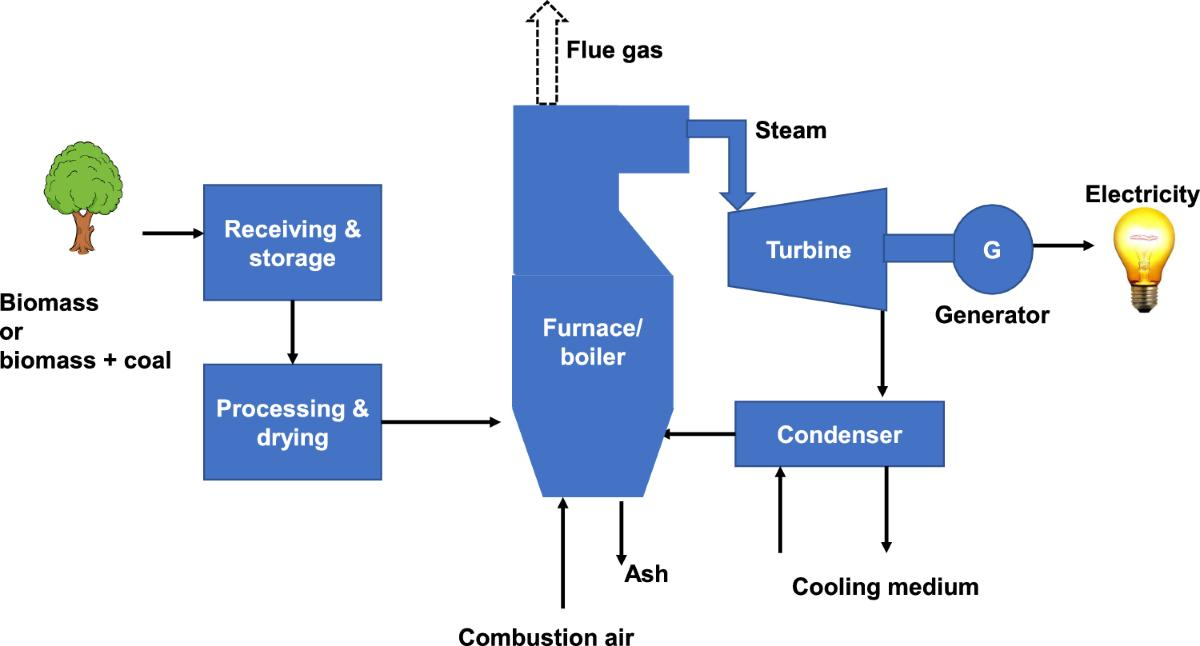
\includegraphics[width=0.9\textwidth]{Figuras/Sección B - Tecnologías de Conversión/Combustión directa - Generación de electricidad.jpg}
    \caption{Esquema de generación eléctrica mediante combustión de biomasa y ciclo Rankine}
\end{figure}

\section{Gasificación}
\label{sec:gasificacion}

La gasificación es la descomposición térmica de la biomasa en una atmósfera reductora de aire, oxígeno o vapor de agua en cantidad subestequiométrica ($\lambda \approx 0{,}2\text{--}0{,}4$) para producir un gas combustible denominado \textit{gas de síntesis} o \textit{syngas} \cite{ieabioenergy2025task33, idae2007gasificacion}. La oxidación parcial aporta el calor necesario para sostener las reacciones de reducción, mayoritariamente endotérmicas.

\subsection{Mecanismo y reacciones principales}
En un gasificador de lecho fijo se distinguen cuatro zonas sucesivas: secado (100--200~\textdegree C), pirólisis (200--600~\textdegree C), oxidación (900--1\,200~\textdegree C) y reducción (700--900~\textdegree C). Las reacciones químicas fundamentales se detallan en la Tabla~\ref{tab:reacciones_gasificacion}.

\begin{table}[htbp]
\centering
\caption{Reacciones principales de la gasificación (entalpías de referencia a 25~\textdegree C).}
\label{tab:reacciones_gasificacion}
\begin{tabular}{@{}llrl@{}}
\toprule
\textbf{Reacción} & \textbf{Ecuación} & \textbf{$\Delta H$ (kJ/mol)} & \textbf{Carácter térmico} \\
\midrule
Combustión completa & $\mathrm{C} + \mathrm{O_2} \longrightarrow \mathrm{CO_2}$ & $-394$ & Exotérmica (aporta calor) \\
Combustión parcial & $\mathrm{C} + \frac{1}{2}\,\mathrm{O_2} \longrightarrow \mathrm{CO}$ & $-111$ & Exotérmica \\
Boudouard & $\mathrm{C} + \mathrm{CO_2} \rightleftharpoons 2\,\mathrm{CO}$ & $+172$ & Endotérmica \\
Agua-gas & $\mathrm{C} + \mathrm{H_2O} \rightleftharpoons \mathrm{CO} + \mathrm{H_2}$ & $+131$ & Endotérmica \\
Desplazamiento (\textit{shift}) & $\mathrm{CO} + \mathrm{H_2O} \rightleftharpoons \mathrm{CO_2} + \mathrm{H_2}$ & $-41$ & Ligeramente exotérmica \\
Metanación & $\mathrm{C} + 2\,\mathrm{H_2} \rightleftharpoons \mathrm{CH_4}$ & $-75$ & Exotérmica \\
\bottomrule
\end{tabular}
\end{table}

\subsection{Agente gasificante, calidad del gas y tipos de reactores}
El agente gasificante determina el poder calorífico del gas obtenido (Tabla~\ref{tab:agente_gasificante}). Con aire, la dilución con nitrógeno reduce el PCI a 4--6~MJ/Nm$^3$ (frente a $\sim 35~\text{MJ/Nm}^3$ del gas natural). El punto de operación habitual con aire se ubica en $\lambda \approx 0{,}25\text{--}0{,}35$: valores inferiores disminuyen la temperatura y aumentan los alquitranes, mientras que valores superiores queman parte del gas producido. La eficiencia de gas frío (\textit{Cold Gas Efficiency}) suele ubicarse entre 65 y 80~\%:
\begin{equation}
\eta_{\text{gas frío}} = \frac{\dot{m}_{\mathrm{gas}} \cdot \mathrm{PCI}_{\mathrm{gas}}}{\dot{m}_{\mathrm{comb}} \cdot \mathrm{PCI}_{\mathrm{comb}}}
\end{equation}

\begin{table}[htbp]
\centering
\caption{Calidad del syngas según el agente gasificante (valores orientativos).}
\label{tab:agente_gasificante}
\begin{tabularx}{\textwidth}{@{}l l X X@{}}
\toprule
\textbf{Agente} & \textbf{PCI del gas} & \textbf{Composición típica} & \textbf{Aplicación} \\
\midrule
Aire & 4--6~MJ/Nm$^3$ & $\mathrm{CO}$ 15--20~\%, $\mathrm{H_2}$ 10--20~\%, $\mathrm{CH_4}$ 1--5~\%, $\mathrm{CO_2}$ 10--15~\%, $\mathrm{N_2}$ 45--55~\% & Motores de combustión interna y calderas; opción más económica. \\
Oxígeno & 10--15~MJ/Nm$^3$ & Libre de $\mathrm{N_2}$; rico en $\mathrm{CO}$ y $\mathrm{H_2}$ & Turbinas de gas y síntesis de combustibles; requiere planta de $\mathrm{O_2}$. \\
Vapor (indirecta) & 12--15~MJ/Nm$^3$ & Libre de $\mathrm{N_2}$; alto contenido de $\mathrm{H_2}$ & Síntesis química y producción de hidrógeno. \\
\bottomrule
\end{tabularx}
\end{table}

Según la configuración hidrodinámica entre biomasa y agente gasificante se distinguen cuatro tipos de reactores (Tabla~\ref{tab:tipos_gasificadores}).

\begin{table}[htbp]
\centering
\small
\caption{Clasificación de reactores de gasificación de biomasa \cite{fao1986woodgas, idae2007gasificacion}.}
\label{tab:tipos_gasificadores}
\begin{tabularx}{\textwidth}{@{}p{2.5cm} p{2.3cm} p{2.1cm} X X@{}}
\toprule
\textbf{Tipo} & \textbf{Flujo} & \textbf{Escala} & \textbf{Ventajas} & \textbf{Limitaciones} \\
\midrule
Lecho fijo \textit{updraft} & Contracorriente & Pequeña & Alta eficiencia térmica; tolera humedad. & Alto contenido de alquitranes; uso térmico directo. \\
Lecho fijo \textit{downdraft} & Co-corriente & Pequeña ($\le 1~\mathrm{MW_e}$) & Craquea los alquitranes; gas apto para motores. & Exige combustible seco y granulometría uniforme. \\
Lecho fluidizado (BFB/CFB) & Arena fluidizada & Mediana a grande & Flexible y escalable. & Alquitranes y partículas intermedios. \\
Flujo arrastrado & Partícula fina ($>1\,200$~\textdegree C) & Muy grande & Gas prácticamente libre de alquitrán. & Requiere molienda intensiva; orientado a síntesis. \\
\bottomrule
\end{tabularx}
\end{table}

El principal obstáculo técnico de la gasificación son los \textbf{alquitranes}, hidrocarburos pesados que condensan al enfriarse y obstruyen filtros, válvulas y motores. Para su uso en motores de combustión interna, el gas debe enfriarse y limpiarse mediante ciclones, filtros, lavadores (\textit{scrubbers}) o craqueo catalítico hasta niveles inferiores a 50--100~mg/Nm$^3$ de alquitrán \cite{fao1986woodgas}. Acoplado a motores de gas (o motores diésel en modo dual), el conjunto alcanza eficiencias eléctricas de 20--30~\%, mientras que la gasificación integrada en ciclo combinado (BIGCC) proyecta 35--45~\%, aunque permanece en fase de demostración \cite{ieabioenergy2025task33}.

\begin{figure}[H]
    \centering
    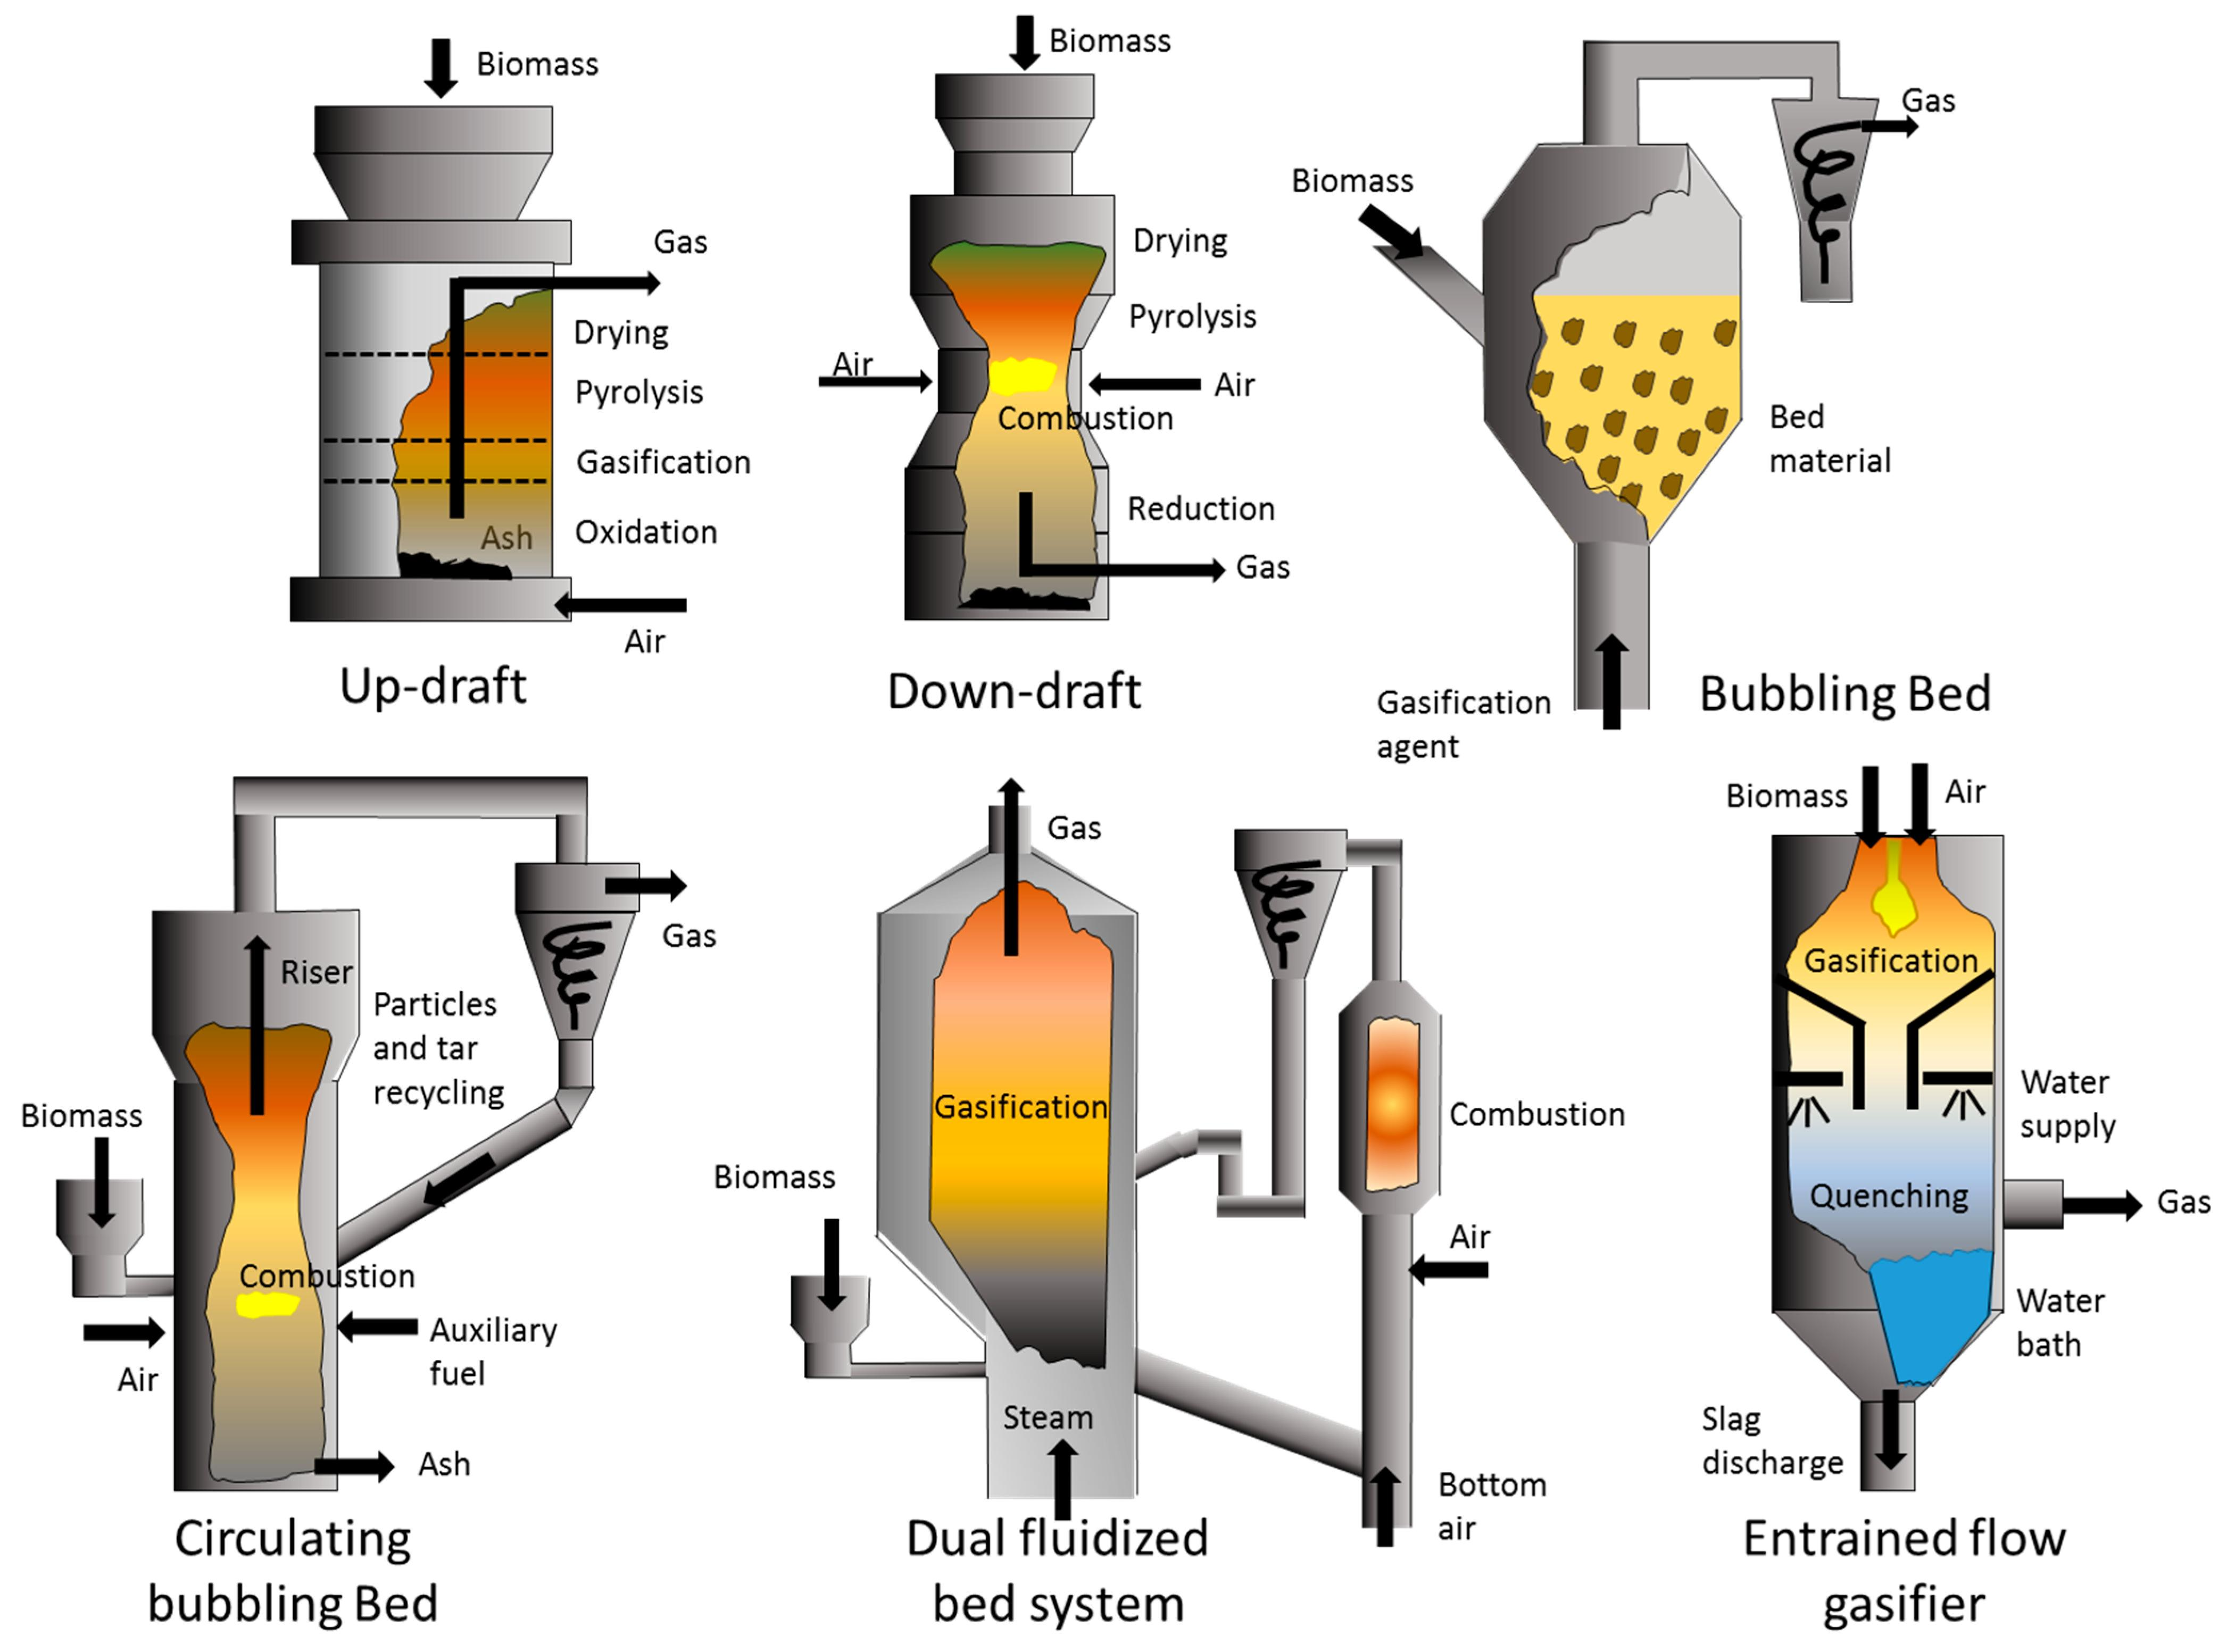
\includegraphics[width=0.8\textwidth]{Figuras/Sección B - Tecnologías de Conversión/Comparación de los tipos de gasificadores.jpg}
    \caption{Comparación esquemática de diferentes configuraciones de gasificadores, incluyendo lecho fijo ascendente (updraft), descendente (downdraft), lecho fluidizado y flujo arrastrado. Se muestran las direcciones de alimentación de biomasa, entrada del agente gasificante y salida del gas producido}
\end{figure}

\begin{figure}[H]
    \centering
    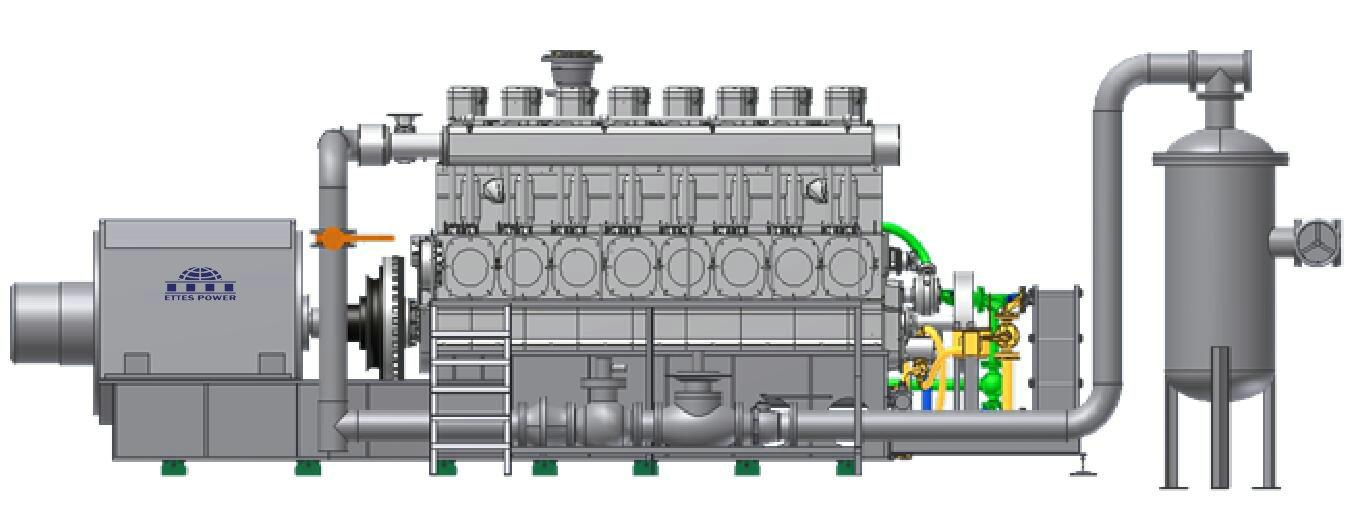
\includegraphics[width=0.8\textwidth]{Figuras/Sección B - Tecnologías de Conversión/Aprovechamiento energético del syngas.jpg}
    \caption{Conjunto motor-generador diseñado para utilizar gas de síntesis como combustible. La combustión del gas dentro del motor produce energía mecánica que acciona un generador eléctrico, permitiendo transformar la energía química del syngas en electricidad}
\end{figure}

\section{Pirólisis}
\label{sec:pirolisis}

La pirólisis es la descomposición térmica de la biomasa en ausencia total de oxígeno ($\lambda = 0$), típicamente entre 300 y 700~\textdegree C \cite{bridgwater2012pyrolysis}. A partir de un balance de masa, la biomasa alimentada se distribuye en tres fracciones: sólida (\textit{biochar}), líquida (\textit{bio-oil} o bioaceite) y gaseosa ($\mathrm{CO}$, $\mathrm{CO_2}$, $\mathrm{H_2}$, $\mathrm{CH_4}$):
\begin{equation}
m_{\mathrm{biomasa}} = m_{\text{bio-oil}} + m_{\mathrm{biochar}} + m_{\mathrm{gas}}
\end{equation}
La proporción relativa depende de la temperatura, velocidad de calentamiento y tiempo de residencia de los vapores (Tabla~\ref{tab:pirolisis_modos}). La pirólisis rápida emplea reactores de lecho fluidizado burbujeante, cono rotatorio o tornillo sinfín con condensación brusca de vapores.

\begin{figure}[H]
    \centering
    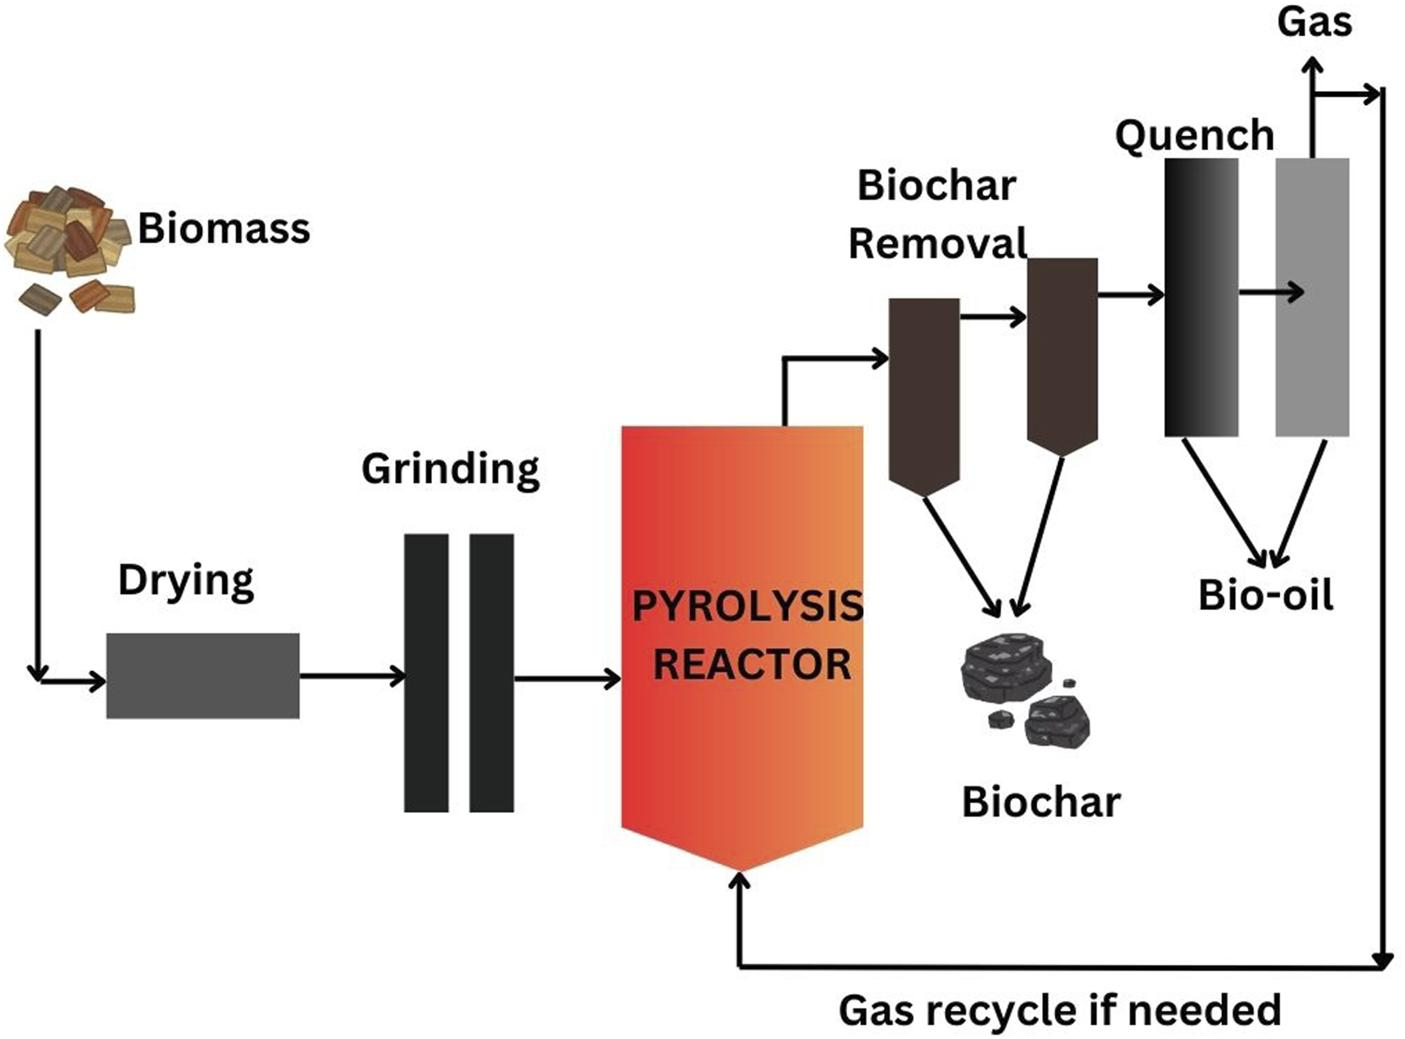
\includegraphics[width=0.8\textwidth]{Figuras/Sección B - Tecnologías de Conversión/Conversón termoquímica - Diagrama de pirólisis.jpg}
    \caption{Diagrama de flujo del proceso de pirólisis de biomasa, incluyendo las etapas de pretratamiento, reacción y separación de productos (biocarbón, bioaceite y gas).}
\end{figure}

\begin{table}[htbp]
\centering
\caption{Distribución típica de productos en pirólisis (porcentaje en masa de biomasa seca) \cite{bridgwater2012pyrolysis}.}
\label{tab:pirolisis_modos}
\begin{tabularx}{\textwidth}{@{}l X ccc@{}}
\toprule
\textbf{Modo} & \textbf{Condiciones típicas} & \textbf{Líquido} & \textbf{Sólido} & \textbf{Gas} \\
\midrule
Lenta (carbonización) & 300--500~\textdegree C; horas a días & $\approx 30~\%$ & $\approx 35~\%$ & $\approx 35~\%$ \\
Intermedia & $\approx 500$~\textdegree C; residencia de vapores 10--30~s & $\approx 50~\%$ & $\approx 25~\%$ & $\approx 25~\%$ \\
Rápida & $\approx 500$~\textdegree C; vapores $\sim 1$~s; enfriamiento brusco & $\approx 75~\%$ & $\approx 12~\%$ & $\approx 13~\%$ \\
Gasificación (ref.) & 750--900~\textdegree C ($\lambda \approx 0{,}2\text{--}0{,}4$) & $\approx 5~\%$ & $\approx 10~\%$ & $\approx 85~\%$ \\
\bottomrule
\end{tabularx}
\end{table}

El valor estratégico de la pirólisis rápida reside en transformar una biomasa voluminosa en un líquido denso y transportable (\textit{bio-oil}), resolviendo parte del problema logístico. Sin embargo, el bioaceite presenta propiedades exigentes frente al fuel oil pesado (Tabla~\ref{tab:biooil}): contiene 15--30~\% de agua, alto oxígeno (35--40~\%), pH ácido (2--3, corrosivo) e inestabilidad por envejecimiento \cite{elliott2017roundrobin}. Por ello, raramente se usa para generación eléctrica directa, empleándose en calderas adaptadas o plantas integradas de cogeneración como Joensuu (Finlandia) y Empyro (Países Bajos) \cite{ieabioenergy_task34}. El \textit{biochar} se destina a enmienda de suelos, secuestro de carbono o combustible sólido.

\begin{table}[htbp]
\centering
\caption{Propiedades típicas del bioaceite de pirólisis rápida frente al fuel oil pesado.}
\label{tab:biooil}
\begin{tabular}{@{}lcc@{}}
\toprule
\textbf{Propiedad} & \textbf{Bio-oil (típico)} & \textbf{Fuel oil pesado (ref.)} \\
\midrule
Poder calorífico inferior & 16--19~MJ/kg & $\approx 40$~MJ/kg \\
Contenido de agua & 15--30~\% & $< 1~\%$ \\
Acidez & pH 2--3 (corrosivo) & Neutro \\
Contenido de oxígeno & 35--40~\% & $\approx 1~\%$ \\
Estabilidad & Envejece (aumenta viscosidad) & Estable \\
Miscibilidad con hidrocarburos & No miscible & --- \\
\bottomrule
\end{tabular}
\end{table}

\section{Digestión anaeróbica}
\label{sec:digestion}

La digestión anaeróbica es un proceso bioquímico en el que un consorcio de microorganismos descompone la materia orgánica en ausencia de oxígeno para producir \textbf{biogás} y un residuo estabilizado rico en nutrientes denominado \textbf{digestato} \cite{alseadi2008biogas, idae2007digestores}. Constituye la ruta idónea para sustratos muy húmedos (estiércoles, lodos de depuradoras, efluentes agroindustriales y fracción orgánica de residuos urbanos), inviables en rutas térmicas \cite{ieabioenergy2024task37}.

\begin{figure}[H]
    \centering
    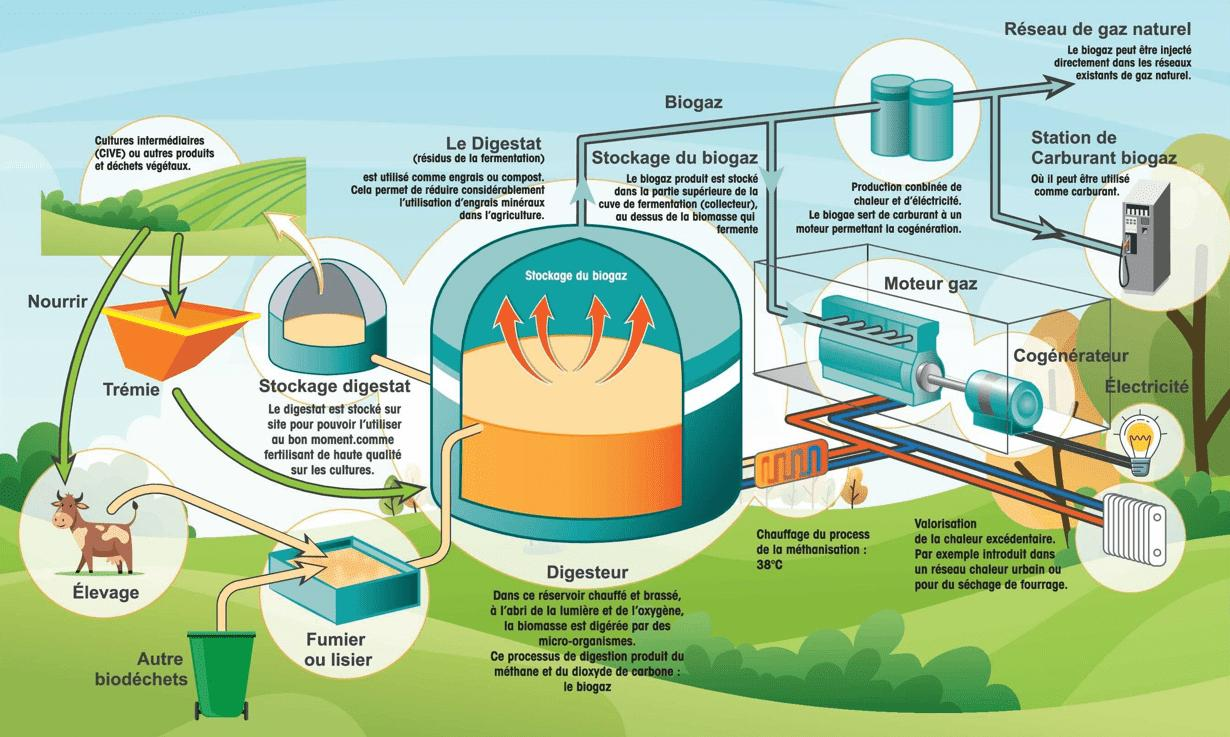
\includegraphics[width=0.8\textwidth]{Figuras/Sección B - Tecnologías de Conversión/Esquema general del proceso de digestión anaeróbica.jpg}
    \caption{Representación de las principales etapas de una planta de digestión anaeróbica, desde la alimentación de residuos orgánicos hasta su descomposición en el digestor}
\end{figure}

\subsection{Etapas y parámetros de operación}
El proceso biológico transcurre en cuatro etapas secuenciales:
\begin{enumerate}[leftmargin=1.5em]
\item \textbf{Hidrólisis:} enzimas extracelulares rompen carbohidratos, proteínas y lípidos en monómeros solubles (etapa limitante en sustratos fibrosos).
\item \textbf{Acidogénesis:} bacterias fermentativas transforman dichos compuestos en ácidos grasos volátiles (AGV), alcoholes, $\mathrm{H_2}$ y $\mathrm{CO_2}$.
\item \textbf{Acetogénesis:} los AGV se convierten en ácido acético, $\mathrm{H_2}$ y $\mathrm{CO_2}$.
\item \textbf{Metanogénesis:} arqueas metanogénicas producen metano por vía acetoclástica ($\sim 70~\%$) e hidrogenotrófica:
\begin{equation}
\mathrm{CH_3COOH} \longrightarrow \mathrm{CH_4} + \mathrm{CO_2}, \qquad \mathrm{CO_2} + 4\,\mathrm{H_2} \longrightarrow \mathrm{CH_4} + 2\,\mathrm{H_2O}
\end{equation}
\end{enumerate}

Los parámetros críticos de control se muestran en la Tabla~\ref{tab:parametros_digestion}. El volumen útil del digestor se dimensiona a partir del caudal diario de sustrato ($Q$) y el tiempo de retención hidráulica ($\mathrm{TRH}$) como $V = Q \cdot \mathrm{TRH}$, operando habitualmente en mezcla completa mesófila con cargas orgánicas volumétricas de 2--5~kg~SV/(m$^3\cdot$día) para evitar la acidificación del reactor.

\begin{table}[htbp]
\centering
\caption{Parámetros de operación de la digestión anaeróbica \cite{alseadi2008biogas, idae2007digestores}.}
\label{tab:parametros_digestion}
\begin{tabularx}{\textwidth}{@{}l l X@{}}
\toprule
\textbf{Parámetro} & \textbf{Valor típico} & \textbf{Importancia operativa} \\
\midrule
Temperatura & Mesófila 30--40~\textdegree C ($\sim 37$~\textdegree C); termófila 50--60~\textdegree C & La termófila acelera la cinética, pero es más inestable y consume mayor calor. \\
pH & 6,5--7,5 & Las arqueas metanogénicas son muy sensibles a la acidificación. \\
TRH & 15--30 días (régimen mesófilo) & Define el volumen útil del digestor. \\
Relación C/N & 20--30 & Un déficit de carbono acumula amoníaco e inhibe el proceso. \\
Inhibidores & Amoníaco, $\mathrm{H_2S}$, exceso de AGV, antibióticos & Pueden reducir o detener la producción de metano. \\
\bottomrule
\end{tabularx}
\end{table}

\subsection{Rendimientos, equipos y tratamiento del biogás}
El biogás contiene 50--70~\% de $\mathrm{CH_4}$ y 30--50~\% de $\mathrm{CO_2}$, más vapor de agua y trazas de $\mathrm{H_2S}$, con un PCI de 20--25~MJ/Nm$^3$. Con 60~\% de metano ($21{,}5~\text{MJ/Nm}^3$), $1~\text{Nm}^3$ equivale a $\sim 6~\text{kWh}$ térmicos, generando $\approx 2\text{--}2{,}3~\text{kWh}$ eléctricos en un motogenerador Otto de 35--40~\% de eficiencia. Los rendimientos varían notablemente según el sustrato (Tabla~\ref{tab:rendimientos_biogas}).

\begin{table}[htbp]
\centering
\caption{Rendimientos orientativos de biogás por tipo de sustrato.}
\label{tab:rendimientos_biogas}
\begin{tabular}{@{}lc@{}}
\toprule
\textbf{Sustrato} & \textbf{Biogás por tonelada fresca (Nm$^3$/t)} \\
\midrule
Estiércol vacuno o porcino & 15--35 \\
Gallinaza & 40--80 \\
Residuos de alimentos / fracción orgánica de RSU & 100--150 \\
Ensilaje de maíz & 170--220 \\
\bottomrule
\end{tabular}
\end{table}

Para ilustrar la escala, un motogenerador de $1~\mathrm{MW_e}$ al 38~\% de eficiencia requiere $1 / 0{,}38 \approx 2{,}63~\mathrm{MW_{th}}$ de biogás ($\approx 440~\text{Nm}^3/\text{h}$ o $10\,600~\text{Nm}^3/\text{día}$ a $21{,}5~\text{MJ/Nm}^3$). Con estiércol a $25~\text{Nm}^3/\text{t}$, ello exige $\approx 420~\text{t/día}$ y un digestor de $V \approx 420 \times 25 \approx 10\,500~\text{m}^3$ ($\mathrm{TRH}=25$~días), razón por la cual estas plantas suelen ser de pequeña escala o recurren a co-digestión. Entre los reactores empleados destacan las lagunas cubiertas (climas cálidos y efluentes agroindustriales), reactores de mezcla completa (CSTR), flujo pistón, reactores UASB (aguas industriales de alta carga) y pozos de captación en rellenos sanitarios.

\begin{figure}[H]
    \centering
    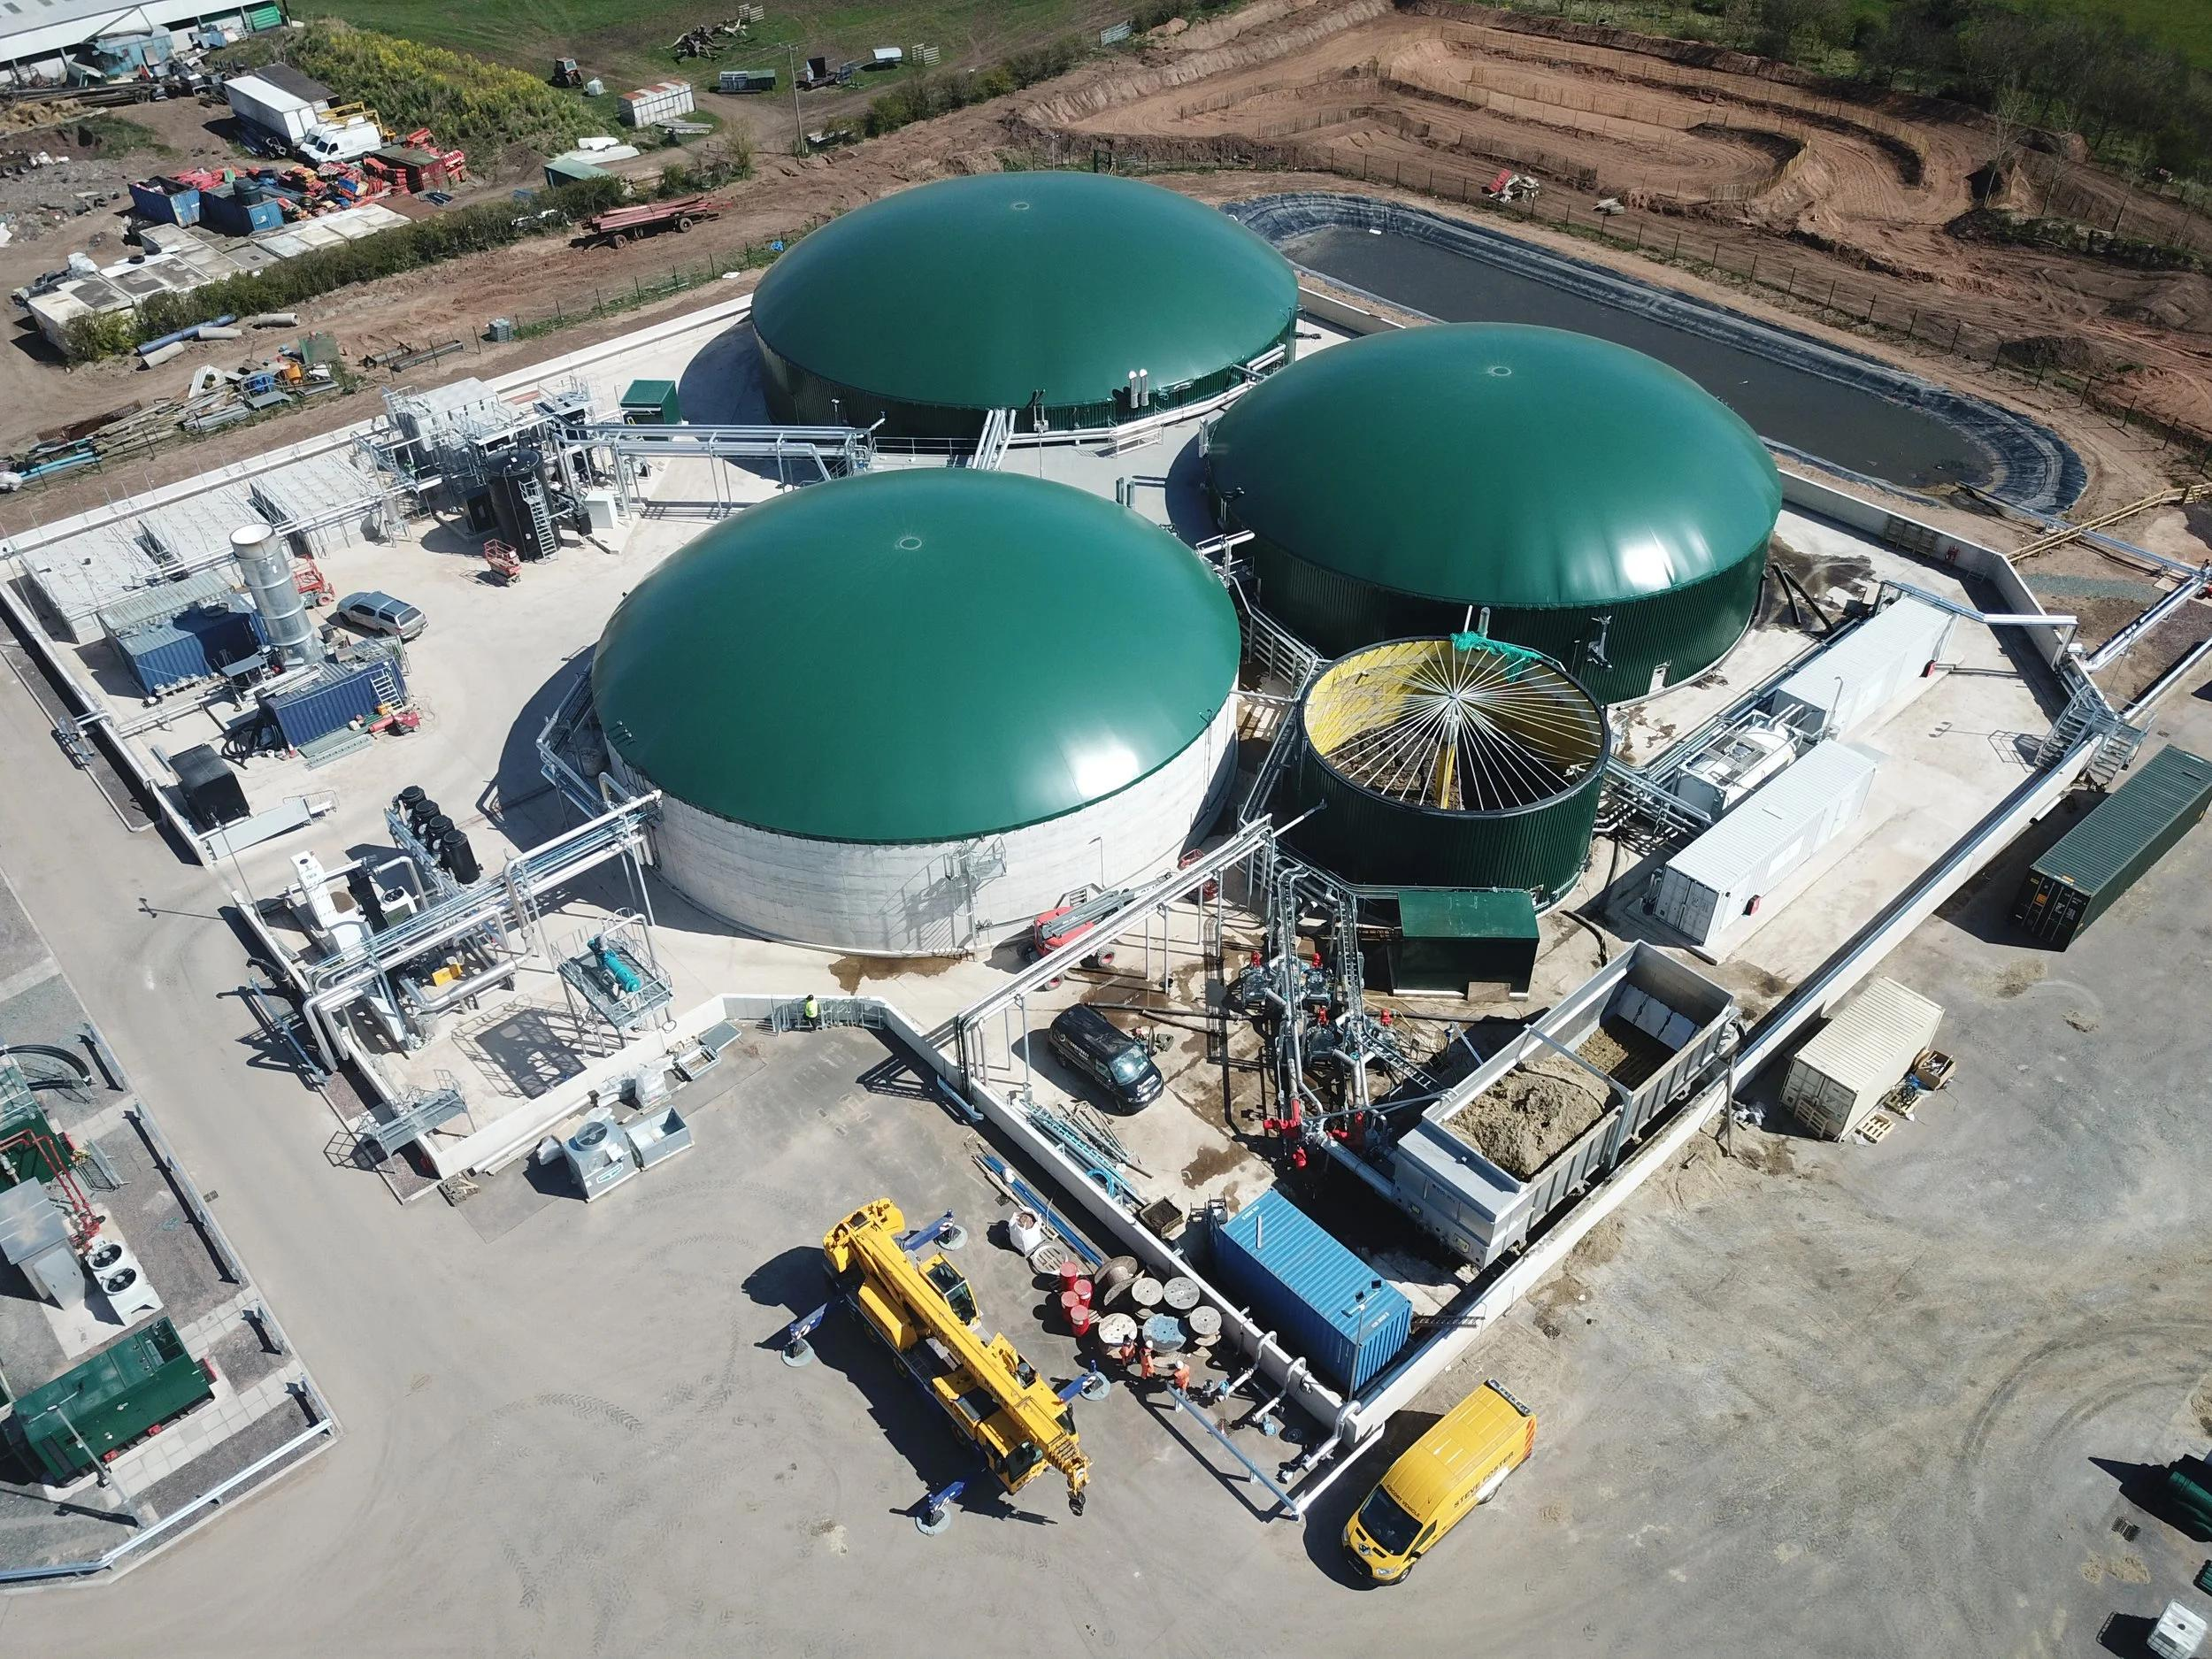
\includegraphics[width=0.8\textwidth]{Figuras/Sección B - Tecnologías de Conversión/Digestores anaeróbicos industriales.jpg}
    \caption{Instalación industrial compuesta por digestores de gran volumen, donde la materia orgánica permanece en condiciones anaeróbicas para favorecer la actividad de los microorganismos metanogénicos. Estos reactores permiten procesar grandes cantidades de residuos orgánicos y producir biogás de manera continua}
\end{figure}

Antes de alimentar motores o inyectarse a red, el biogás se seca y desulfura (para remover el $\mathrm{H_2S}$ corrosivo y siloxanos en gas de relleno). Mediante separación de $\mathrm{CO_2}$ (lavado con agua, PSA o membranas) se obtiene \textit{biometano} ($>95~\%~\mathrm{CH_4}$). La IEA estima un potencial global sostenible cercano a $10^{12}~\text{m}^3$ equivalentes de gas natural al año, del cual hoy se aprovecha menos del 5~\% (1,76~EJ en 2023) \cite{iea2025biogas, wba2025gbsr}.

\section{Comparación de rutas para generación eléctrica}
\label{sec:comparacion_rutas}

La Tabla~\ref{tab:comparacion_rutas} sintetiza el desempeño eléctrico, la escala típica y la madurez comercial de las distintas tecnologías analizadas. No existe una opción universalmente superior: la combustión con ciclo Rankine domina en mediana y gran escala con biomasa sólida; la gasificación y el ORC atienden nichos descentralizados; y la digestión anaeróbica con motogeneradores lidera en residuos húmedos.

\begin{table}[H]
\centering
\caption{Comparación de sistemas de generación eléctrica con biomasa (valores orientativos).}
\label{tab:comparacion_rutas}
\begin{tabularx}{\textwidth}{@{}X l l l@{}}
\toprule
\textbf{Sistema de generación} & \textbf{Escala típica} & \textbf{$\eta$ eléctrica} & \textbf{Madurez} \\
\midrule
Caldera + turbina de vapor (Rankine), dedicada & 5--300~$\mathrm{MW_e}$ & 20--35~\% & Comercial madura \\
Co-combustión en central de carbón & $>100~\mathrm{MW_e}$ & 36--44~\% \cite{irena2013cofiring} & Comercial \\
Caldera + ciclo Rankine orgánico (ORC) & 0,2--5~$\mathrm{MW_e}$ & 15--20~\% & Comercial \\
Gasificador + motor de combustión interna & 0,1--pocos $\mathrm{MW_e}$ & 20--30~\% & Comercial (exige limpieza) \\
Gasificación integrada en ciclo combinado (BIGCC) & $>20~\mathrm{MW_e}$ & 35--45~\% (proy.) & Demostración \\
Biogás + motogenerador & 0,05--5~$\mathrm{MW_e}$ & 35--42~\% (s/biogás) & Comercial madura \\
Pirólisis + motor o turbina & --- & --- & Precomercial \\
\bottomrule
\end{tabularx}
\end{table}

\begin{figure}[H]
    \centering
    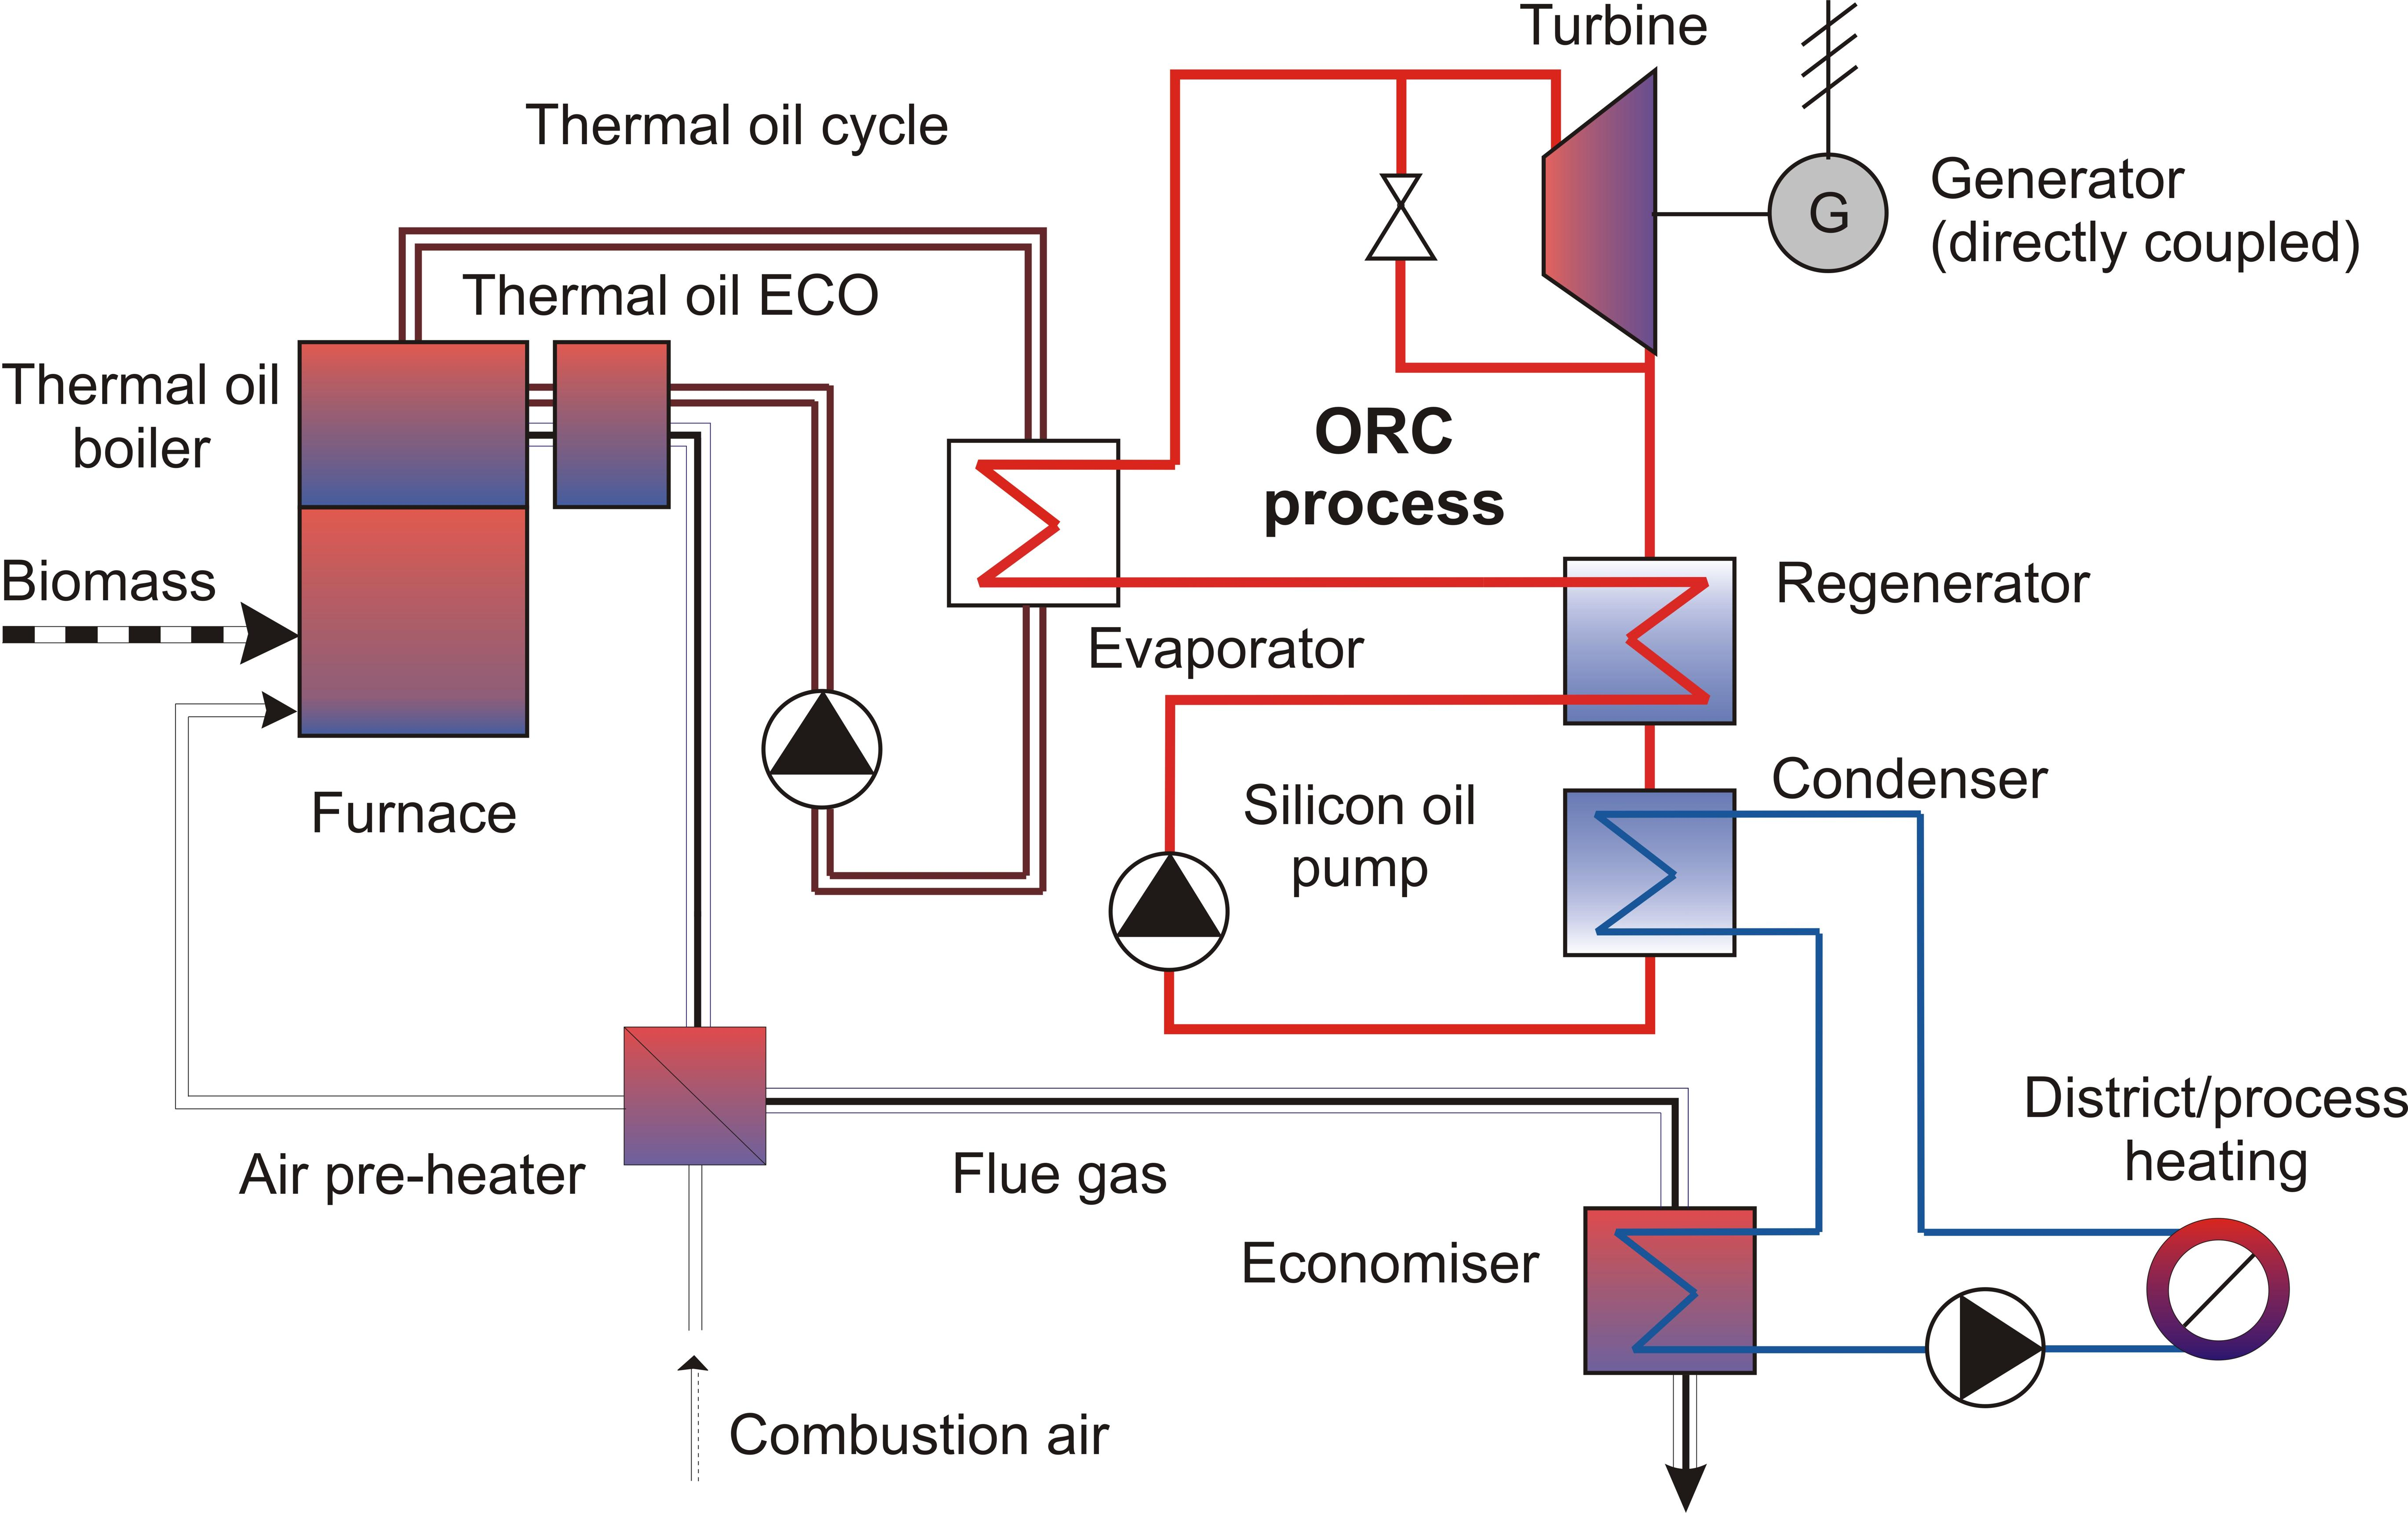
\includegraphics[width=0.9\textwidth]{Figuras/Sección B - Tecnologías de Conversión/Generación eléctrica mediante ciclo Rankine orgánico (ORC).jpg}
    \caption{Generación eléctrica mediante ciclo Rankine orgánico (ORC): El calor procedente de una fuente térmica se transfiere a un fluido orgánico de bajo punto de ebullición. El vapor generado acciona una turbina conectada a un generador eléctrico y posteriormente se condensa para retornar al evaporador, cerrando el ciclo. Esta tecnología permite aprovechar fuentes de calor de temperaturas relativamente bajas}
\end{figure}

\begin{figure}[H]
    \centering
    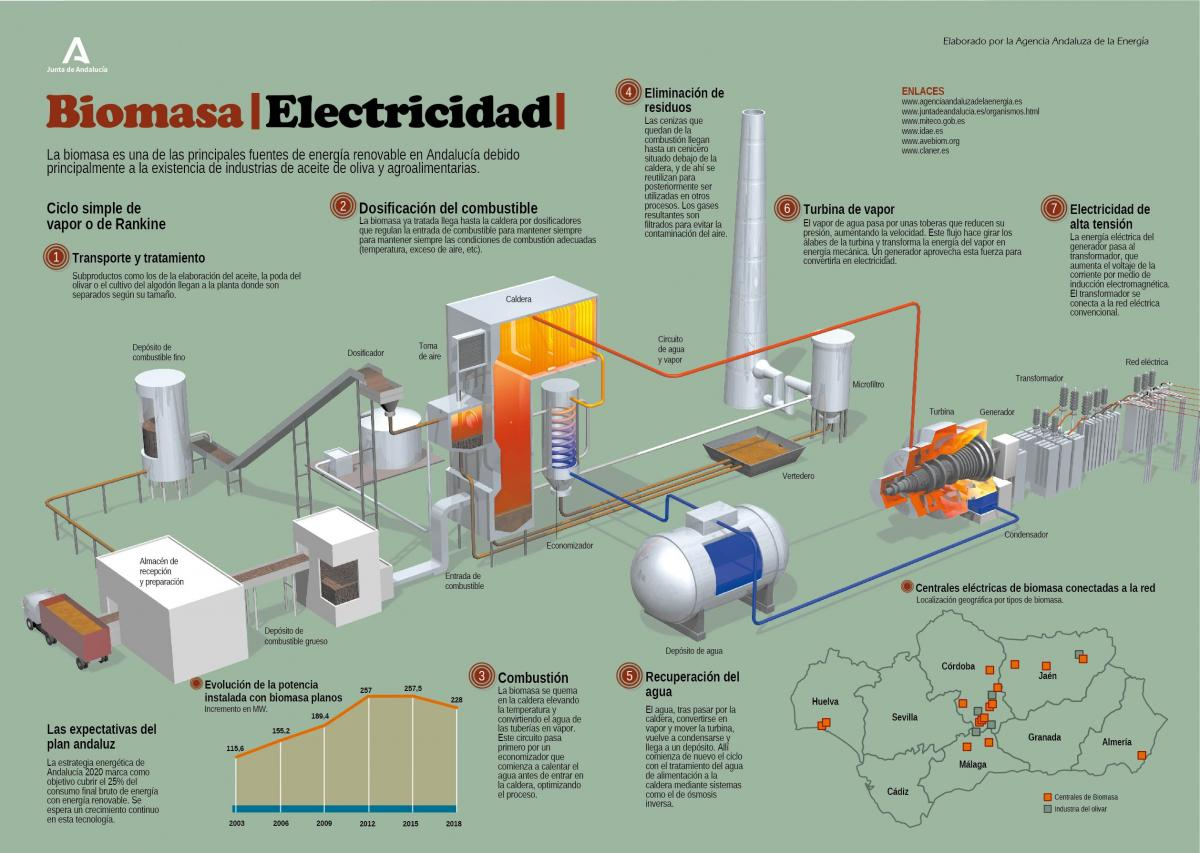
\includegraphics[width=0.75\textwidth]{Figuras/Sección B - Tecnologías de Conversión/Generación eléctrica mediante combustión directa y ciclo Rankine.jpg}
    \caption{Generación eléctrica mediante combustión directa y ciclo Rankine: Sistema de generación eléctrica en el que la biomasa sólida se quema en una caldera para producir vapor de agua a alta presión y temperatura. Este vapor se expande en una turbina acoplada a un generador eléctrico, mientras que posteriormente se condensa y recircula para completar el ciclo termodinámico}
\end{figure}

\begin{figure}[H]
    \centering
    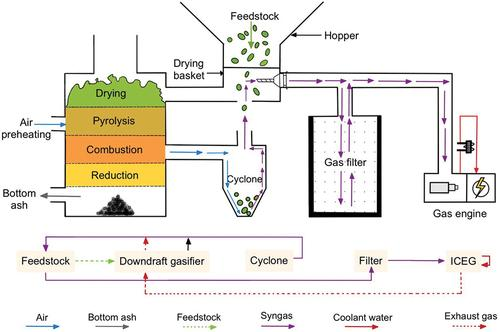
\includegraphics[width=0.75\textwidth]{Figuras/Sección B - Tecnologías de Conversión/Gasificación de biomasa para generación eléctrica.jpg}
    \caption{Gasificación de biomasa para generación eléctrica: Proceso de conversión termoquímica de biomasa sólida en un gas combustible mediante su reacción a temperaturas elevadas con una cantidad controlada de agente gasificante. El gas producido, compuesto principalmente por monóxido de carbono, hidrógeno y metano, pasa por un sistema de acondicionamiento y limpieza antes de alimentar un motor de combustión interna acoplado a un generador eléctrico}
\end{figure}

\begin{figure}[H]
    \centering
    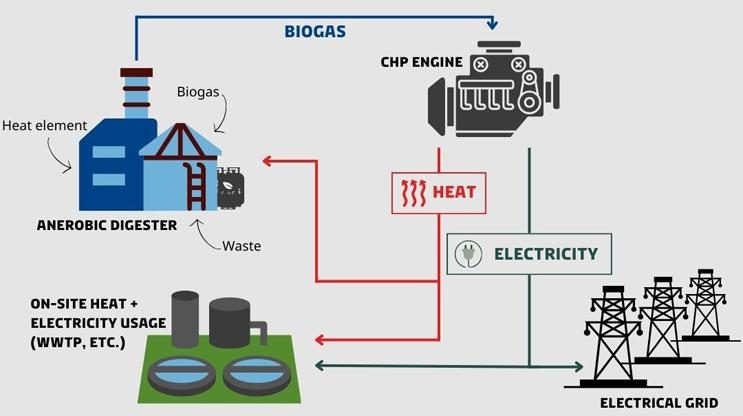
\includegraphics[width=0.8\textwidth]{Figuras/Sección B - Tecnologías de Conversión/Generación eléctrica mediante biogás y ciclo de cogeneración.jpg}
    \caption{Generación eléctrica mediante biogás y ciclo de cogeneración: Utiliza el biogás producido en un digestor anaeróbico como combustible para alimentar un motor de combustión interna acoplado a un generador eléctrico. Además de producir electricidad, el sistema recupera el calor residual de los gases de escape y del circuito de refrigeración del motor para su aprovechamiento térmico, incrementando la eficiencia energética global de la instalación}
\end{figure}

En términos de selección tecnológica, la viabilidad de cada ruta depende principalmente de las características del recurso biomásico, su disponibilidad, contenido de humedad, poder calorífico y escala de aprovechamiento, así como de los requerimientos de inversión y operación. También deben considerarse la eficiencia energética global, los sistemas de pretratamiento y acondicionamiento del combustible y la posibilidad de recuperar el calor residual mediante cogeneración. Por tanto, la elección debe responder a un análisis técnico-económico que contemple tanto el rendimiento de conversión eléctrica como los costos de instalación, mantenimiento, suministro de biomasa y gestión de subproductos. En general, la integración de tecnologías de conversión con sistemas de recuperación energética permite mejorar el aprovechamiento del recurso y reducir las pérdidas, favoreciendo la viabilidad de los proyectos de generación eléctrica a partir de biomasa.

Adicionalmente, el desarrollo de estas tecnologías representa una alternativa para diversificar la matriz energética y reducir la dependencia de los combustibles fósiles, especialmente en regiones con disponibilidad constante de residuos agrícolas, forestales, ganaderos y agroindustriales. Sin embargo, su implementación requiere garantizar un suministro sostenible de materia prima, establecer sistemas eficientes de recolección y transporte y controlar las emisiones generadas durante la conversión. De esta manera, la generación eléctrica con biomasa no solo debe evaluarse por su capacidad de producir energía, sino también por su contribución al aprovechamiento de residuos, la economía circular y la sostenibilidad ambiental a largo plazo.
